\documentclass{article}
\usepackage{amsfonts}
\usepackage{amsmath}
\usepackage{amsthm}
\usepackage{amssymb}
\usepackage{enumitem}
\usepackage{xcolor}
\usepackage{graphicx}
\usepackage{caption}
\usepackage{csquotes}
\usepackage{fontawesome}
\usepackage{hyperref}
\usepackage{geometry}
 \geometry{
 a4paper,
 left=30mm,
 right=30mm,
 }
\usepackage{url}
\usepackage{setspace}

\newcommand\longvar[1]{\mathchardef\UrlBreakPenalty=100
\mathchardef\UrlBigBreakPenalty=100\url{#1}}

\newcommand{\aaa}[2]
	{\href{#1}{#2}}
	
\everydisplay{\def\arraystretch{0.5}}

\title{KWS2102 Term 1 Report\\Sobel Operator VHDL Implementation\\Repo: \aaa{https://github.com/slypiggies/fyp}{\faGithub}}
\author{Lam Kin Long (1155127407)}
\date{}
\begin{document}
	\renewcommand{\baselinestretch}{2}\normalsize
\begin{titlepage}
\maketitle\thispagestyle{empty}
\end{titlepage}
	\begin{abstract}
		In this paper, a field-programmable gate array (FPGA) system for edge detection has been developed. This system allows in \textbf{real-time}, finding edges from a live video stream in VGA 640x480 resolution. Edges of objects with distinct background colors are highlighted in white. The system uses the Xilinx ZedBoard with the XC7Z020 system on a chip (SoC) as the main processing unit, a single camera sensor OV7670 for video acquisition, and VGA \cite{vga} for video output. The system is coded in the hardware description language (HDL) VHDL, developed on the Xilinx Vivado software suite, and lays out the foundation for future object detection work. Possibilities include the detection of 2D data codes, such as QR codes and AprilTags.
	\end{abstract}\newpage
	
	\renewcommand{\baselinestretch}{1.88}\normalsize
	\tableofcontents
	\renewcommand{\baselinestretch}{2.35}\normalsize
	
	
	\newpage\section{Technical Background for the Report}
	\subsection{FPGA}
		Field-programmable gate arrays (FPGAs) are hardware that can be reprogrammed to achieve logic functions. As opposed to a CPU (central processing unit), FPGAs do not take instructions, and execute them one by one. It is simply a cluster of logic blocks designed to be modified to perform highly specific task. Building circuits manually with logic gates, e.g., using a breadboard, can also achieve this exact same behavior, however with an FPGA changes can be done a lot quicker, and for complicated designs mistakes can be avoided. FPGA is also more flexible than building circuits manually, because practically there are an infinite amount of logic gates on it (Figure \ref{zynq7020}).
	\begin{figure}[h]
		\centering
		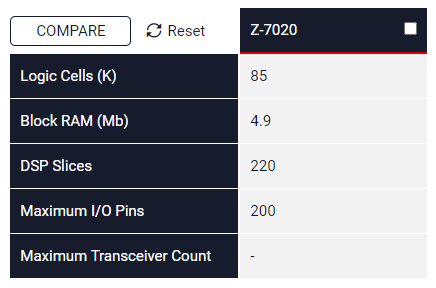
\includegraphics[scale=1]{zynq7020}
		\caption{The specification of the FPGA chip on the ZedBoard, with 85K logic cells.}
		\label{zynq7020}
	\end{figure}
		\\
		
		FPGAs are good for systems which require high data throughput, because these different I/Os can be programmed to connect to logic blocks directly to perform the specific task. If these tasks are executed by a CPU, the instructions will need to wait to be executed sequentially, and so a slower response time. Another major difference between an FPGA and a CPU is the amount of pipelining an FPGA can achieve. Within a clock cycle, there can be multiple things happening at the same time, such as a camera giving a pixel and another pixel being handled by logic blocks (Figure \ref{fig:pipelining}).
	\begin{figure}[h]
		\centering
		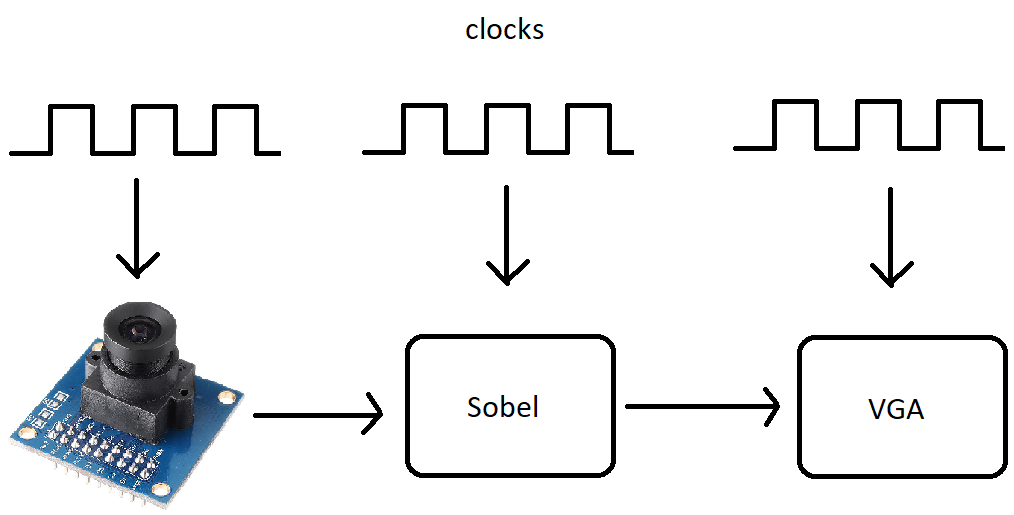
\includegraphics[scale=0.45]{pipelining}
		\caption{Different components from the project are running in pipeline, a form of parallelism. They do not need to wait for the prior component to finish before starting their own task.}
		\label{fig:pipelining}
	\end{figure}
	\\
	
	But for CPUs, the amount of instructions pipelining can no longer be flexible as the chip is manufactured already. It cannot be hardware-reprogrammed to do things other than executing instructions. 
	\\
	
		In theory, one can design a CPU on an FPGA, as CPU is nothing but a circuit with different components connected together. This type of CPU is being called as a soft core, because the design of this CPU can be modified with a reprogram. The other type of CPU, hard core, is the one that one will typically find in a computer, and the internal circuits can no longer be modified.
		
	\subsection{HDL}
		FPGAs are typically programmed in hardware description languages (HDLs), and the one being used in this project is called VHDL. HDLs are not programming languages, they do not produce instructions being runned by a CPU. Instead, they infer circuits that match the logic behaviors described by the code. For example, the statement \texttt{C <= (not A) and (A or B)} will infer logic that matches the following figure (Figure \ref{fig:circuit1}).
	\begin{figure}[h]
		\centering
		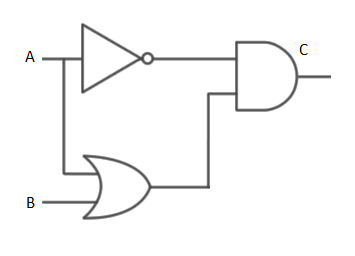
\includegraphics[scale=0.6]{circuit1}
		\caption{A circuit with a not-gate, and-gate and an or-gate.}
		\label{fig:circuit1}
	\end{figure}
	The circuit in this figure is called asynchronous circuit, as the output, in this case \texttt{C}, can be uniquely determined by the values of the input, in this case \texttt{A} and \texttt{B}. 
	\\
		
		Another type of circuits is called synchronous circuit. For this type of circuit, the output not only depends on the inputs, but also on time and the previous state. This previous state is being stored in a storage element, known as a flip-flop. For example, the following code \begin{displayquote}
			\texttt{if rising\_edge(clock) then Q <= D}
		\end{displayquote} will infer a circuit that transfers the content from register \texttt{D} to register \texttt{Q}, only if the the clock is rising. The circuit representing this logic is shown in (Figure \ref{fig:dff}).
	\begin{figure}[h]
		\centering
		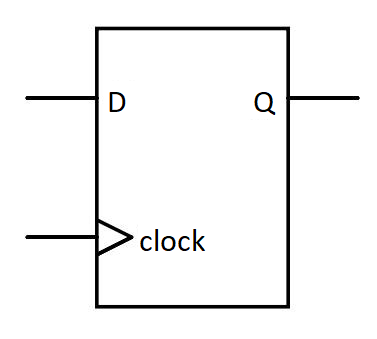
\includegraphics[scale=0.35]{dff}
		\caption{The circuit with a single flip-flop}
		\label{fig:dff}
	\end{figure}For what a flip-flop is, please refer to \aaa{https://circuitdigest.com/electronic-circuits/d-flip-flops}{this link}, as it makes the whole introduction too long to fit within these short backgrounds.
	\\
		
		The transformation from HDL to circuits is known as synthesis. It is analogous to compilation in the software world. Synthesis is not only responsible for the transformation, it also optimizes the circuit such that it meets timings. This process is known as place and route. This is required, because in practice signal across logic gates experiences a predictable amount of delay. And, there may be two sets of circuits that behave the same functionally but one with faster paths (Figure \ref{fig:twolevel}).
	\begin{figure}[h]
		\centering
		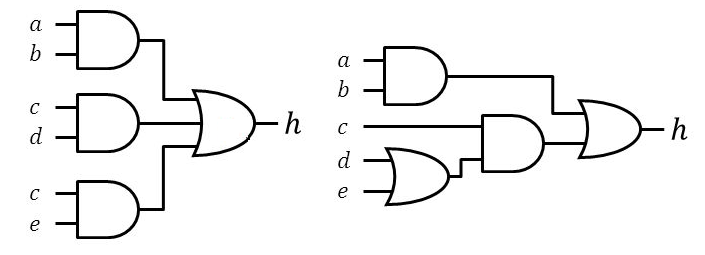
\includegraphics[scale=0.6]{twolevel}
		\caption{Two circuits with identical behavior. However, the one on the left has better timing, as any path in the circuit only needs to go through at most 2 logic gates. Paths in the right circuit may need to go through 3 logic gates, thus 3 delays.}
		\label{fig:twolevel}
	\end{figure}
	\\
		
		Note that timing in the current project has already been violated (Figure \ref{fig:timing}).
	\begin{figure}[h]
		\centering
		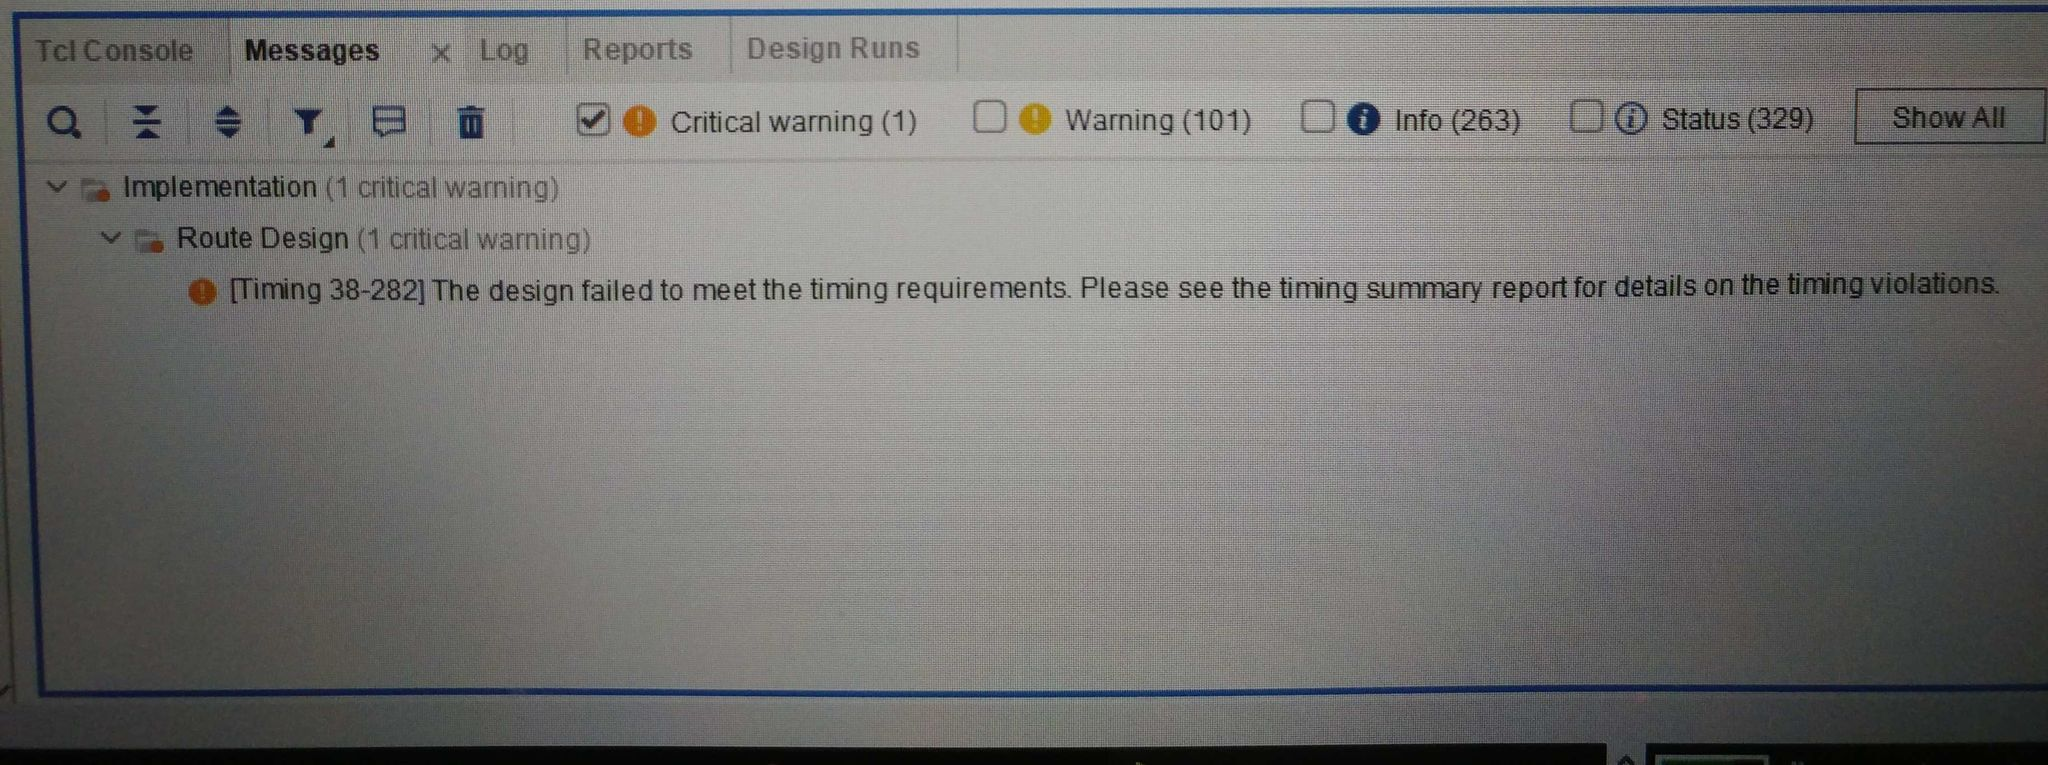
\includegraphics[scale=0.2]{timing}
		\caption{The failed timing from Vivado}
		\label{fig:timing}
	\end{figure}But it has no visible effect yet, and I also do not know how to fix it.
	
	\subsection{Serial Communication}
		To transfer data between devices, serial communication protocols are used. These protocols specify how the devices involved should react upon receiving electrical signals. Some protocols also have special functionalities, such as error-correction. For the protocol used in this project, it does not have these abilities, so they are not explained in detail.
	\\
		
		Any synchronous serial communication protocols use at least 2 wires, namely clock and data. The clock facilitates how fast the data should be sent, or received. These two wires also act together to signal the beginning of a transfer, and the end of a transfer.
	\\
		
		For the protocol used in this project, the start condition is indicated by the following waveform diagram, Figure \ref{fig:wavewave}. That is, serial data (SDA) will be pulled low when serial clock (SCL) is still high. The end condition will be similar, but in reverse. Also, typically a device cannot endure an SCL that is too fast. Otherwise, the transfer speed of the protocol can reach infinity, as imagined.
	\\
		
	\begin{figure}[h]
		\centering
		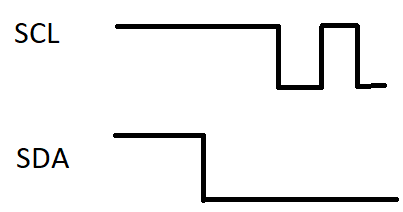
\includegraphics[scale=0.5]{wavewave}
		\caption{The starting condition of the protocol used in this project, SCCB.}
		\label{fig:wavewave}
	\end{figure}
		
		The maximum frequency of SCL of an device can typically be found in its data sheet.
		
	\subsection{VGA}
		Video graphics array (VGA) means a couple things. It can mean the display output protocol, the physical connector, or the standard resolution 640x480. The following waveform diagrams describe how VGA looks like (Figure \ref{fig:vgaline}, \ref{fig:vgaframe}).
	\begin{figure}[h]
		\centering
		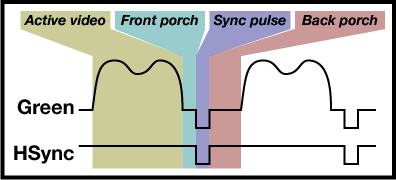
\includegraphics[scale=0.8]{vgaline}
		\caption{The waveform diagram of VGA for a single line}
		\label{fig:vgaline}
	\end{figure}
	\begin{figure}[h]
		\centering
		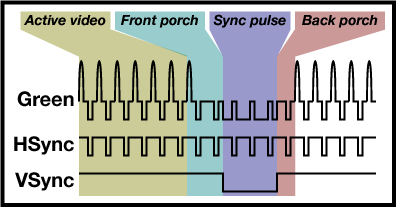
\includegraphics[scale=0.8]{vgaframe}
		\caption{The waveform diagram of VGA for a single frame, i.e., multiple lines}
		\label{fig:vgaframe}
	\end{figure}
	\\
	
	The HSync pulse is responsible for telling the display (in the old days, cathode ray tube (CRT) displays) that the next horizontal line is coming. During the period around the HSync, known as front porch, sync pulse and back porch, the display output is disabled and the RGB signal line should remain black. For CRTs, this period is for the electron gun to move to the beginning of the next line, shown in Figure \ref{fig:scanline}.
	\begin{figure}[h]
		\centering
		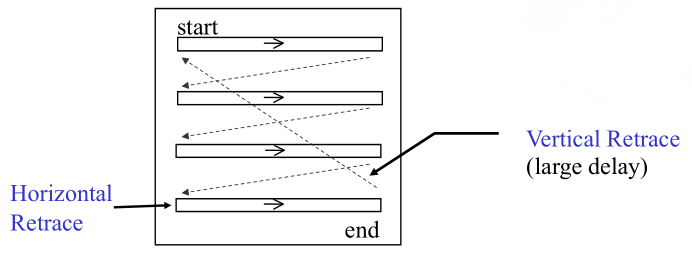
\includegraphics[scale=0.78]{scanline}
		\caption{The electron gun moving back horizontally when it reaches the end of a line}
		\label{fig:scanline}
	\end{figure}
	Similarly, when a frame is finished, this VSync pulse should occur, and porch around that pulse also exist, that the host should only transmit black pixels, i.e., all zeroes.
	\\
		
		Different resolutions should have different amount of time for the porches and the pulses. They are specified by the VGA standard, as shown in the table (Figure \ref{fig:vgatiming}).
	\begin{figure}[h]
		\centering
		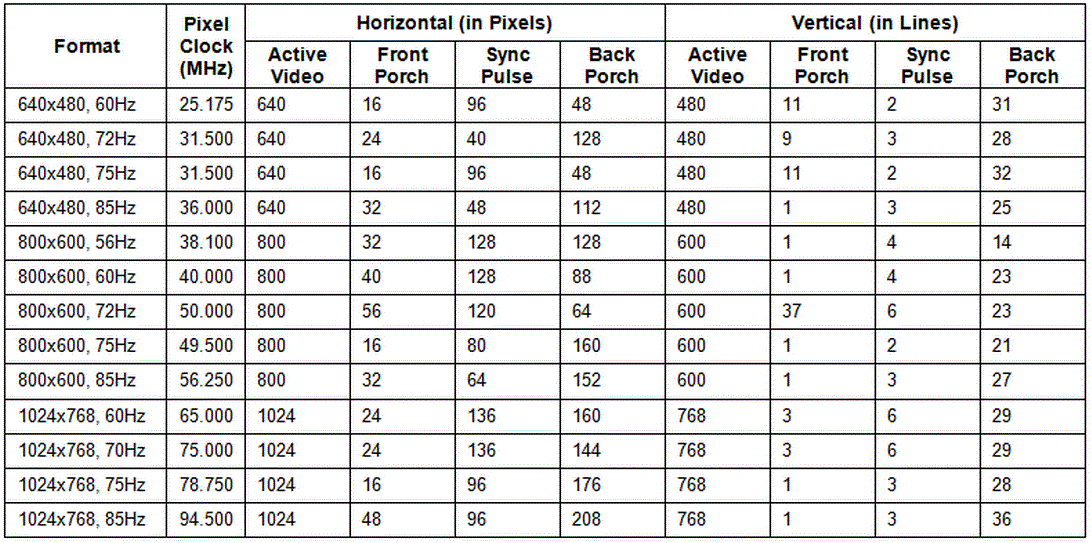
\includegraphics[scale=0.5]{vgatiming}
		\caption{The partial specification table of the VGA parameters. The resolution used in this project is corresponding to the first entry.}
		\label{fig:vgatiming}
	\end{figure}
	\\
		
		For the VGA physical connector, the picture is shown in Figure \ref{fig:vgacon}.
	\begin{figure}[h]
		\centering
		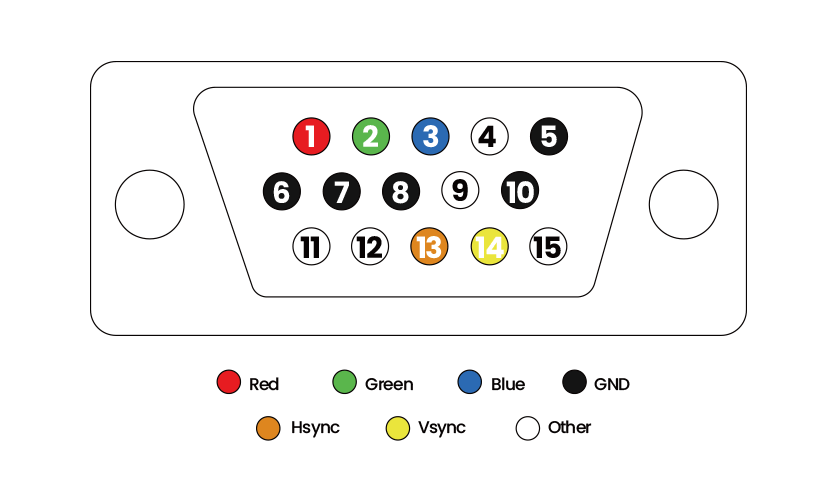
\includegraphics[scale=0.31]{vgacon}
		\caption{The VGA connector}
		\label{fig:vgacon}
	\end{figure}While there are pins for advanced usages, five pins are used in this project. They are the HSync pin, VSync pin, red, green and blue pin. The synchronization pins are in digital, and the RGB pins are in analog.
	\\
		
		For the VGA connector used in the project, the RGB pins are wired additionally to a 4-to-1 digital to analog converter (DAC). 4-to-1 means that an analog pin will now only have 2\textsuperscript{4} = 16 possibilities, instead of infinity that true analog can provide.
	\\
		
		In layman's terms, each pixel in the current system is represented in a 12-bit value, 4-bit per color channel. This enables the control of the VGA protocol by the FPGA used, because it can simply sends digital 0s or 1s to the pins of the DAC.
		
	\subsection{Edge Detection}
		Edge detection means highlighting edges from a real-world image, and non-edge pixels will stay black. As shown in Figure \ref{fig:edge1} and \ref{fig:edge2} ,
	\begin{figure}[h]
		\centering
		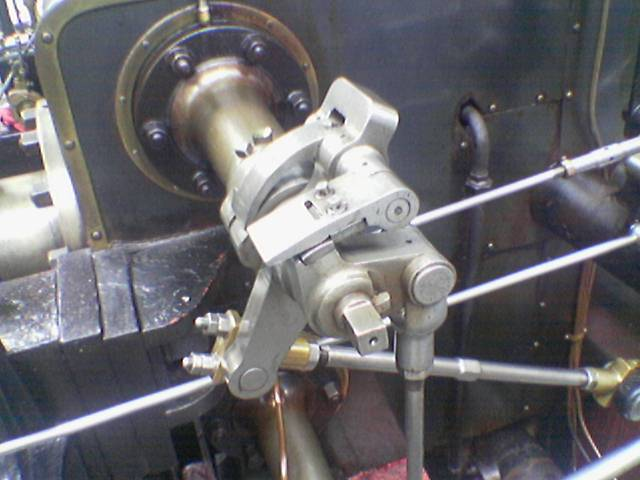
\includegraphics[scale=0.52]{edge1}
		\caption{Original Image}
		\label{fig:edge1}
	\end{figure} 
	\begin{figure}[h]
		\centering
		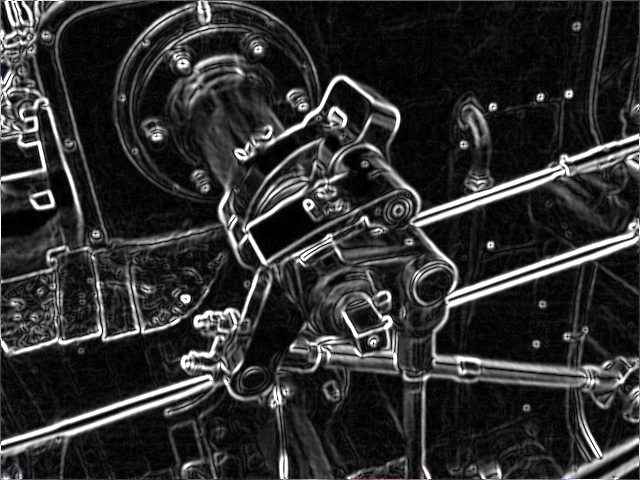
\includegraphics[scale=0.52]{edge2}
		\caption{Edge detected image}
		\label{fig:edge2}
	\end{figure}pixels that are part of an edge is highlighted. Therefore, edge detection is taking a picture as input, and output another picture with the exact same resolution.
	\\
	
	In this project, this resolution is the resolution of standard VGA, 640x480. There are different techniques for obtaining edges from an image, notably ones that are based on convolution with a 2D matrix.
	
	\subsection{Convolution}
		Convolution, represented by $*$, is a mathematical operation that operates on 2D data. It takes two matrices, one of them called as the kernel, for the following operation (assume the left matrix is the kernel, the right are the pixels to be convoluted):
		\begin{align*}
			\begin{pmatrix}
				a&b&c\\
				d&e&f\\
				g&h&i
			\end{pmatrix} * 
			\begin{pmatrix}
				j&k&l\\
				m&n&o\\
				p&q&r
			\end{pmatrix}=
			aj+bk+cl+dm+en+fo+gp+hq+ir
		\end{align*}
		Here, $n$ is the pixel that is being focused on, but as illustrated in the equation pixels around $n$ will also be brought into consideration. Each pixel is treated with the above convolution matrix, so that for each pixel there will be nine multiplications. All the pixels in the 640x480 should be treated with this process, and edges in the frame should be specially handled (Figure \ref{fig:boundary}),
	\begin{figure}[h]
		\centering
		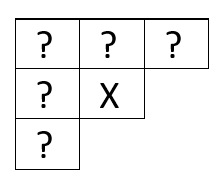
\includegraphics[scale=0.9]{boundary}
		\caption{For the upper-left corner pixel X, neighbors out of boundary are marked with a ?.}
		\label{fig:boundary}
	\end{figure} mentioned later.
		For edge detection, there are two popular kernels. They are Canny's and Sobel's respectively. For this project, Sobel kernel is chosen (which will be in more detail later), because the concept of a 3x3 matrix doing convolution is commonly seen in a lot of image processing tasks, not only edge detection, and the whole edge detection system will be very useful for future 2D image object recognitions. On the contrary, Canny's is a 2x2 matrix, and due to it not being used in this project, its descriptions are omitted.
	\\
		
		Note that in the following paragraphs, the kernel itself will represent the result of a convolution involving that kernel, as an notation abuse. Otherwise the notations will get confusing.
		
	\subsection{Sobel Operator}
	Sobel operator is used for detecting edges. As for why Sobel is chosen instead of other methods for edge detection, and more detailed information such as implementation, it will be revisited in later sections. Sobel operator consists of two kernels,
	\begin{align*}
		G_x&=
		\begin{pmatrix}
			1&0&-1\\
			2&0&-2\\
			1&0&-1
		\end{pmatrix},\\
		G_y&=
		\begin{pmatrix}
			1&2&1\\
			0&0&0\\
			-1&-2&-1
		\end{pmatrix}.
	\end{align*}
	The input picture will be convoluted, pixel by pixel, by the above two kernels. So two pixel values will be obtained for each pixel. To form the resultant pixel $G$, the two values will be combined, using the formula
	\begin{align*}
		G&=\sqrt{{G_x}^2+{G_y}^2}.
	\end{align*}
	The rationale behind $G_x$ and $G_y$ is derivatives, which is a concept which deals with the rate of change. For $G_x$, it is horizontal, and for $G_y$, it is for vertical. For horizontal derivatives, it should be the value of the larger X minus by that of smaller X. Which means, the following formula for $G_x$ should make more sense:
	\begin{align*}
		G_x&=
		\begin{pmatrix}
			-1&0&1\\
			-2&0&2\\
			-1&0&1
		\end{pmatrix}.
	\end{align*}
	This is also true for $G_y$. However, the former definition (which the positives and the negatives are swapped) are used, just to stick with the definition from the Sobel article from Wikipedia. These two definitions do not actually matter in the end, as the results are squared anyway.
	
	The reason for the middle row/column to be 2 instead of 1, is to put more emphasis on the current row/column being processed.
	
	Again, more details can be found later.
		
	\newpage\section{Introduction}
	One of the most challenging problems which robots face is how they can align themselves with the outside world. If the robots are not controlled manually, they will need to use sensors to perceive ambient parameters. Unless the terrains are specifically designed for the robots, they cannot rely on primitive techniques like tracing black lines. While humans can simply use their eyes to locate where they are, robots need to detect specialized objects, realistically recognized within a very short and bounded amount of time. This is known as \emph{real-time}.
	\\
	
	That's where the significance of FPGA comes into play, and the fundamental reason why other alternatives are not being used -- FPGA can achieve data processing in the measure of clock-cycles. For the specialized 2D data code AprilTags (Figure \ref{fig:apriltag}),
	\begin{figure}[h]
		\centering
		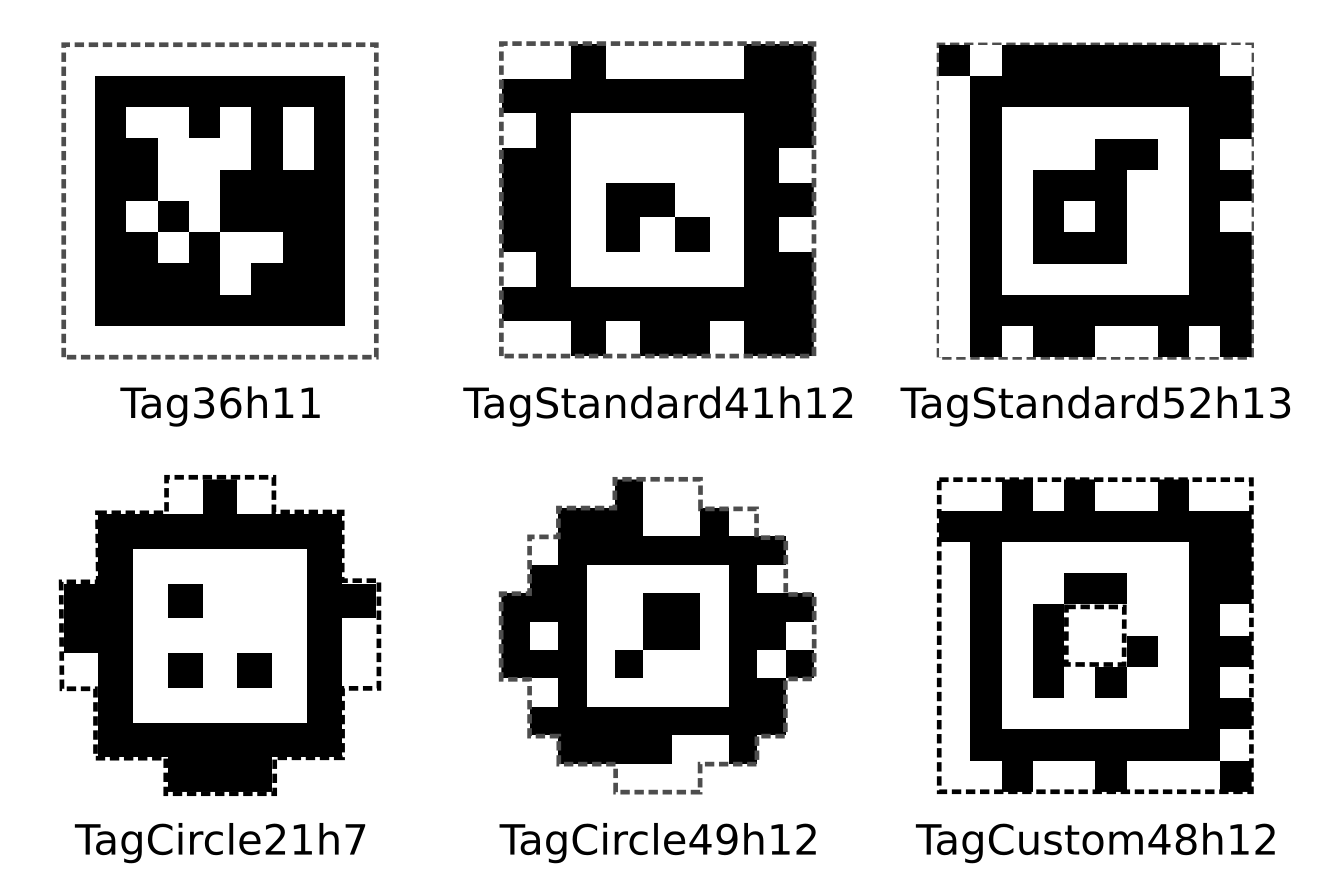
\includegraphics[scale=0.2]{apriltag}
		\caption{Examples of different AprilTags.}
		\label{fig:apriltag}
	\end{figure}
	\\
	
	the first step of code detection involves edge detection. For other 2D codes such as QR codes and DataMatrices, the first steps may differ. It shows the edge detection is a prevalent problem and highly fundamental, which is good for setting up the overall system and for me to be familiar with FPGAs and VHDL. It also lays out the foundation of work in the next semester, something more advanced than edge detection.
	\section{Significance}
		Robot navigations are the most challenging issue that robots need to deal with today. Moreover, robots need to react within a short, and bounded amount of time. In this project, an FPGA system on edge detection has been developed, such that it can detect edges from a video source, \emph{in real time}.
	\\

		Edge detection is closely related to object recognition. For example, AprilTag is designed for this purpose, and the first step of recognizing it has to do with recognizing the edges of the code. Moreover, the Sobel operator was chosen, because it involves a 3x3 matrix in convolution with the image. This operation is very commonly seen in image processing, and the idea is that if this cannot be done with my FPGA skill level, no further image processing task can ever be done. Also, the whole system developed for this 3x3 convolution work will be very useful for future work, as any other 3x3 convolution operation simply requires a change of parameters to the current system. A lot of hardware-related problems can also be avoided in the future, as they have been heavily dealt with in the current project.
	\newpage\section{Electronics Used in the Project}
	FPGA is chosen for the task because of its large amount of I/O. It is also inherently good at achieving deep pipelining, as discussed in the previous section Technical Background. Large parallelism can also be achieved on an FPGA, if it is being programmed explicitly to do so. For example, if the registers to be transferred are explicitly programmed to be very wide.
	\\
	
	The ZedBoard (Figure \ref{fig:zedboard}) is chosen due to it being available from the laboratory. It also includes useful connectivities, Pmod and VGA.
	\begin{figure}[h]
		\centering
		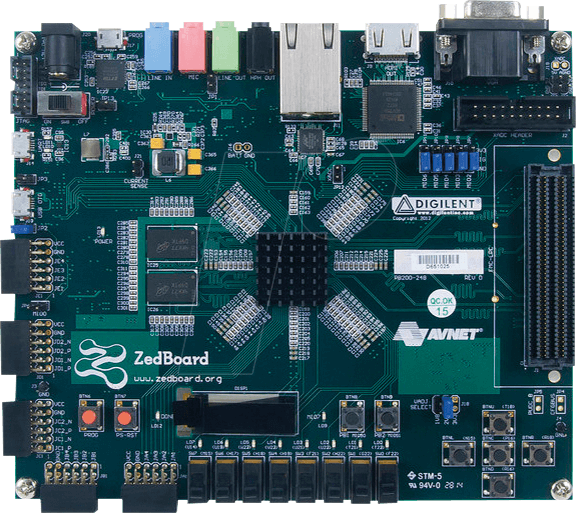
\includegraphics[scale=0.6]{zedboard}
		\caption{Xilinx ZedBoard}
		\label{fig:zedboard}
	\end{figure}
	\\
	
	\subsection{Why FPGA is better than ASIC} Compared to an application-specific integrated circuit (ASIC), FPGA is better for prototyping because of it being reconfigurable. ASIC on the other hand, is fixed, and very expensive to manufacture, even though it can be more efficient than an FPGA. ASIC is typically for designs that have already been tested with FPGAs.
	\\
	
	\subsection{Why not traditional form of processors}
	Two other obvious alternatives include microcontrollers (MCU) and single-board computers (SBC).
	\\
	
	The on-board oscillator of a popular MCU, Arduino Uno, can only go up to 16 MHz, which is slower than just the pixel clock from the camera. It also only has 22 available pins, which assuming can all be used simultaneously, are still barely enough for the current system \footnote{The current system uses 16 pins for the camera, 5 pins for VGA (3 of them, RGB, being analog), 1 pin for reset, excluding any power and ground pins}. More powerful MCUs may be suitable for the current system’s application, but they leave little room for future expansions, compared to FPGAs.
	\\
	
	For SBCs, online demo shows that a Raspberry Pi 3B+ can process only up to 10 FPS \cite{rpi}, just by doing edge detection alone. Moreover, most SBCs run Linux, instead of a real-time operating system, and in theory the response time of a non real-time operating system cannot be guaranteed.
	\\
	
	Unless more power-hungry and expensive computers with dedicated graphics are considered, FPGA is the better choice.
	\begin{figure}[h]
		\centering
		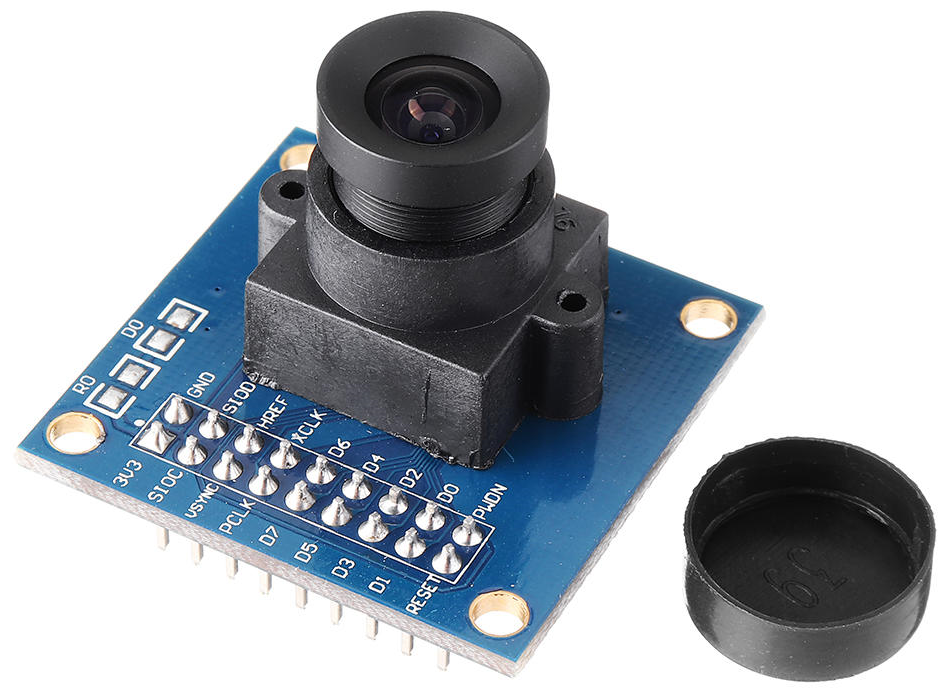
\includegraphics[scale=0.2]{ov7670}
		\caption{OmniVision OV7670}
		\label{fig:ov7670}
	\end{figure}
	\\
	
	For the camera sensor, OV7670 from OmniVision (Figure \ref{fig:ov7670}) \cite{ovdatasheet} has been chosen, due to it being easy to control (or so I thought). It is also a very cheap sensor, which is good for embedded applications. It can achieve up to 30 FPS with the standard VGA resolution (Figure \ref{fig:officialadv}),
	\begin{figure}[h]
		\centering
		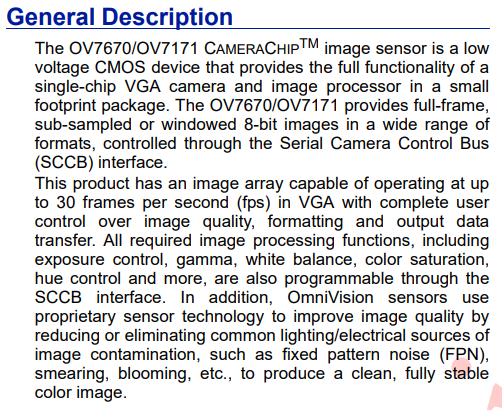
\includegraphics[scale=0.7]{officialadv}
		\caption{The complete description of OV7670 from the manufacturer}
		\label{fig:officialadv}
	\end{figure} connected to the Pmod I/O (Figure \ref{fig:pmod})
	\begin{figure}[h]
		\centering
		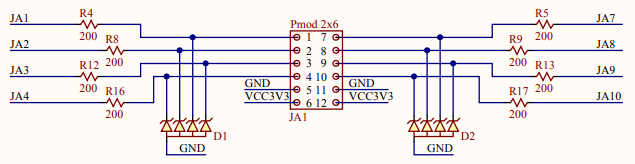
\includegraphics[scale=0.87]{pmod}
		\caption{The Pmod pinout of ZedBoard}
		\label{fig:pmod}
	\end{figure} of the ZedBoard. Pmod I/O is simply treated as general-purposed I/O (GPIO) in this project. Similarly, VGA has been chosen for the video output interface due to its low complexity.
	\\
	
	In the following sections, the overall architecture of the current system is introduced. After that, each component is explained in more detail. Finally, some difficulties encountered are presented.
	\newpage\phantom{blabla}
	\newpage\section{Project Progress}
	
	\subsection{August}
		An FPGA was borrowed back in May, but August is the month when I started working on the project. I could not start earlier due to an internship. In this month, I revised the topic of digital systems, such as flip-flops and finite state machine implementation.
	\\
		
		After that, some background knowledge on FPGAs was learnt from the internet, as I did not know anything about the topic despite having interest. Then I quickly started learning my first HDL, VHDL, using the book \emph{Free Range VHDL}. It really confused me in the beginning, due to me always accidentally treating it as a programming language, thus not understanding the examples in the book. The whole book was finished before the semester formally started. It provided me knowledge for my first HDL, and in hindsight I do not think one can learn HDL simply from the internet without at least finishing a book, unlike programming languages.

	\subsection{Week 1}
		In this week, the actual topics was discussed. The conclusion was to use FPGA to detect some kind of 2D data code, such as QR code. But until today I am still not sure if QR code, or some other 2D data matrix decode can be handled by my level of FPGA knowledge. Maybe some other object detection will be more viable.
	\\
		
		Also, Xilinx Vivado, the synthesis software for the FPGA, was downloaded, and license was asked from the technician. This software is so large ($>$50 GB) that I needed to delete something from the hard disk in order to fit it. After setting up the software, I tried programming the FPGA with VHDL code, but I was producing syntax-valid yet un-synthesisable circuits. I also produced some code that can work in theory, but cannot work on the physical FPGA due to the architecture of the particular FPGA that I was using. That specific example is not included here.
		
		Then, it was understood what patterns to avoid, e.g., putting a non-clock signal (button signal for example) inside \texttt{rising\_edge()} (i.e., do not do \texttt{rising\_edge(button)}), when I needed to code VHDL.
	
	\subsection{Week 2 to Week 3}
		In these weeks, papers and videos on object recognition using an FPGA were read and watched. Strangely, no paper on QR code decode using an FPGA was found, probably due to the fact that no one has successfully developed a working system for this application yet. Nonetheless the structures of QR code, DataMatrix code were understood, even though they are not useful in the current project, which I could not foresee back then.
	\\
		
		Moreover, different cameras have been considered, but in the end the OV7670 sensor was chosen because it is supposedly easy to control, cheap, and available from the lab. The existing FPGA on my hand, the ZCU102, has also been swapped to the ZedBoard due to it lacking a Pmod connector with compatible dimensions and the lack of a VGA port.
	\\
		
		The VGA protocol has also been understood, which is actually formally taught during Week 8 of the course CENG3430 rapid prototyping. But I did not take the course, thus lacking formal education on the matter. The code has been developed for the protocol. But the design needs to be tested in the lab due to me lacking a VGA monitor at home, so the permission to enter the lab was requested and the lab has been regularly visited.
	\\
		
		Anecdotally, One night I could not reenter the lab after going out for toilet, as at that time there was no one remaining in the building who could help me. So the personal belongings were left there overnight and picked up in the next day.
	
	\subsection{Week 4}
		In this week, the code for the camera has finally been prepared, and after a lot of troubleshooting, including swapping multiple sensors, there was finally something to be seen on the VGA monitor. Even though the image was not in good condition. (I did not take photo for this, sorry). At this point, my understanding on the camera was still not adequate, in hindsight. Also, it was discovered suddenly that the lab has some portable VGA displays available for borrowing, so one has been picked up, and the lab was no longed needed to be visited.
	
	\subsection{Week 5 to Week 7}
		In this weeks, issues around the camera has been dealt, which will be revisited in the Difficulties section. This sensor, while being cheap, has just been hard to work with. The data sheet has been spotted with a lot of errors, and numerous configurations has been tested. Notice that at this point, ``actual work'' (ones that would be expected from a non-FPGA project, from anyone not worked with FPGAs before) has not been started. Just a lot of work that can be neglected from the progress point of view.
	\\
		
		Eventually, the whole SCCB protocol has to be re-understood, which is responsible for the transmission of the camera configurations. A testbench testing the transmission of register configuration has been developed, to ease the tracking of bugs and issues not related to my work.
	
	\subsection{Week 8 to Week 9}
		In this weeks, edge detection could finally be started, the idea being any object detection work will not be far from matrices convolution, and it would be a good exercise due to it being so fundamental, that if it cannot be done then no other work can ever be done, by my FPGA skill level. The system involving edge detection has been designed, which involves a controller and a convolutor component (more in the Implementation section). Code has been developed really quickly for these components. However, there have been a long time which no output could simply be seen, and another testbench was developed to see the behavior of these two components working together. Eventually, the problem was tracked down to again, the camera, that the speed of the SCCB protocol was too fast, some particular register settings cannot be successfully transmitted to the camera.
	
	\subsection{Week 10 to the end}
		The output of the edge detection can finally be seen, but with a lot of noise and unwanted artifacts. It has not been understood initially, if the problem was originating from the quality of the camera, from the registers, or from the logic of the components that I developed. After time-consuming investigations, I was convinced that the camera quality has been the culprit for the noise. Therefore, multiple workarounds have been thought and developed and tested, and some will be visited in the later section Implementation.
	\newpage\section{System Architecture}
	\begin{figure}[h]
		\centering
		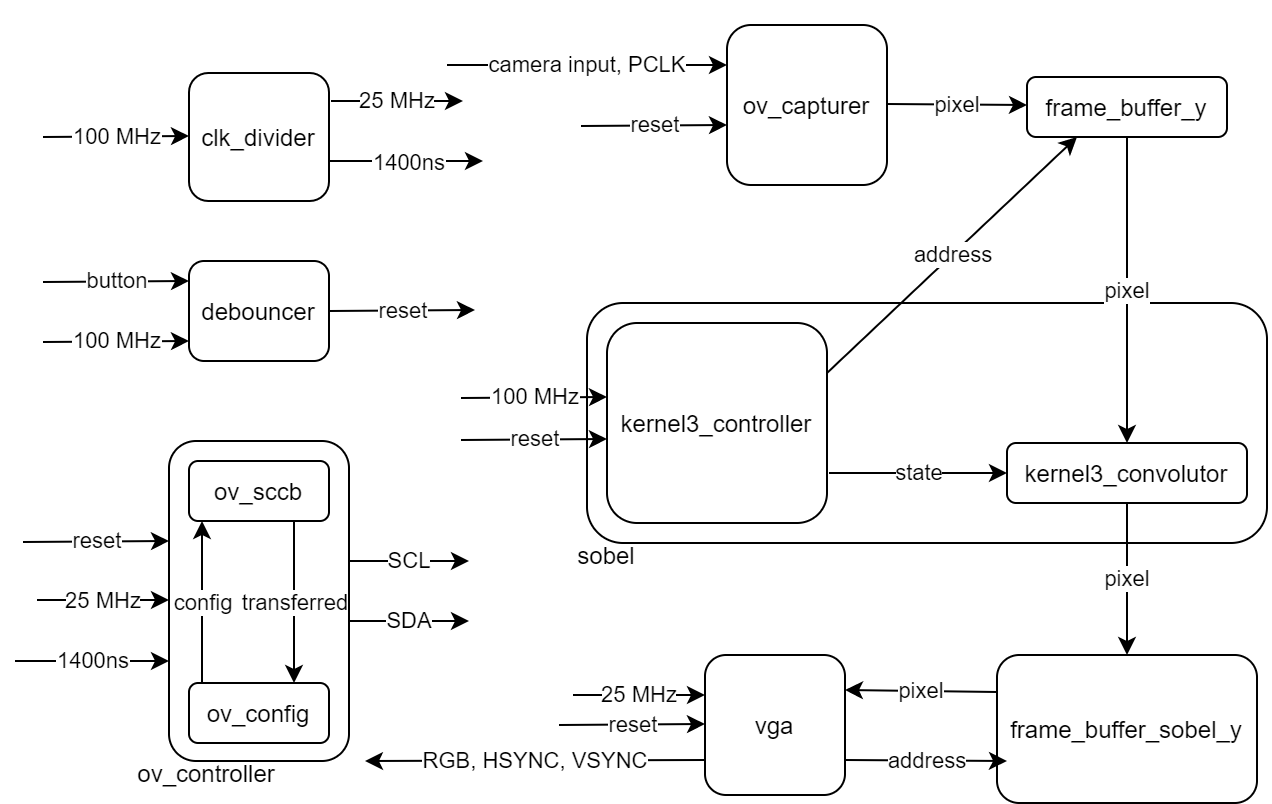
\includegraphics[scale=0.42]{block}
		\caption{Block Diagram}
		\label{fig:block}
	\end{figure}
	Figure \ref{fig:block} shows the top level design of the current system, which has already been simplified from the actual system. There are 10 components in total, including 2 frame buffers.
	\\
	\begin{enumerate}
		\item \texttt{clk\char`_divider} is responsible for taking a fast clock input, and generate a clock that is slower than the input by factors of multiples.
		\item \texttt{debouncer} is responsible for stabilizing button inputs. The output will only be 1 if the input has stayed 1 for a certain amount of time.
		\item \texttt{ov\char`_sccb} is responsible for configurating the camera. Without the configuration, the camera looks so bad, that one may be misled that the camera is faulty.
		\item \texttt{ov\char`_config} stores the values of the registers to be sent. Once \texttt{ov\char`_sccb} finishes sending a register, it notifies \texttt{ov\char`_config} to provide the next one, until all registers have been sent.
		\item \texttt{ov\char`_capturer} interfaces incoming data from the camera, and puts it into the first frame buffer \texttt{frame\char`_buffer\char`_y} (Y stands for the luma (brightness) component in the YUV color space).
		\item \texttt{kernel3\char`_controller} provides coordinates for each clock. These coordinates go to \texttt{frame\char`_buffer\char`_y}, and the returned pixel is fed to the \texttt{kernel3\char`_convolutor}.
		\item \texttt{kernel3\char`_convolutor} is running in synchronous to \texttt{kernel3\char`_controller}. For each clock cycle, it is supposed to receive a pixel in the 3x3 convolution matrix (the Sobel kernel for the current system), then do the multiplication with addition. Therefore, for every 9 cycles a pixel result should be formed. This result is fed to the next frame buffer (\texttt{frame\char`_buffer\char`_sobel\char`_y} for the current system).
		\item \texttt{vga} is responsible for generating the video output signal, by taking pixels from the last frame buffer.
	\end{enumerate}
	\newpage\section{Implementation Details}
	\begin{figure}[h]
		\centering
		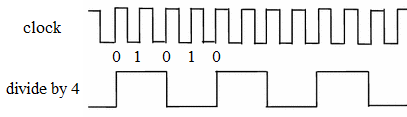
\includegraphics[scale=0.8]{clockdivider}
		\caption{The bottom clock toggles when the counter reaches 0}
		\label{fig:clockdivider}
	\end{figure}
	\texttt{clk\char`_divider} and \texttt{debouncer} are the easiest to implement. Both utilizes a counter. For \texttt{clk\char`_divider}, the counter is increased by one when there is a positive edge, and the output clock toggles if this counter has reached a particular threshold, illustrated in Figure \ref{fig:clockdivider}. The clock divider is needed, as various components in the other parts of the system, requires clock with slower frequency. For example the VGA protocol required a clock with 25 MHz.
	\\
	
	For \texttt{debouncer}, for each clock the state of the button is checked. The \texttt{debouncer} output will be 1 only if the button has been pressed for certain consecutive numbers of clock. \texttt{debouncer} is required because of the mechanical nature of the button, it tends to micro-vibrate when it is being pressed and released. The reset button is currently being wired to this \texttt{debouncer}, otherwise the reset will toggle between 0 and 1 constantly for a short burst, something that the camera cannot handle. The camera needs a settling time of 1 ms between each reset, shown in (Figure \ref{fig:setllingtime}).
	\begin{figure}[h]
		\centering
		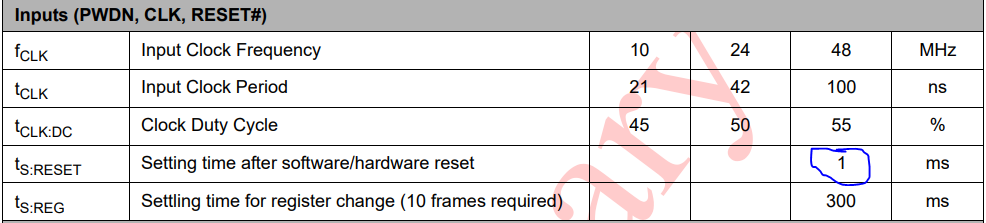
\includegraphics[scale=0.55]{setllingtime}
		\caption{From the datasheet, the camera needs a settling time of 1 ms after being resetted.}
		\label{fig:setllingtime}
	\end{figure}
	
	\begin{figure}[h]
		\centering
		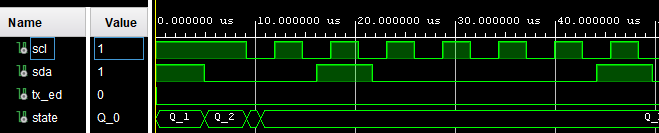
\includegraphics[scale=0.83]{sccb1}
		\caption{Start condition of SCCB. The first byte being transferred is 0x42, the SCCB address of OV7670}
		\label{fig:sccb1}
	\end{figure}
	\begin{figure}[h]
		\centering
		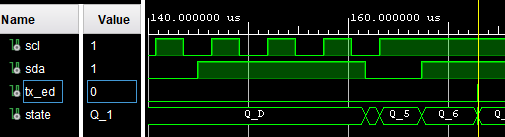
\includegraphics[scale=0.83]{sccb2}
		\caption{End condition of SCCB: SDA being pulled high while SCL is high}
		\label{fig:sccb2}
	\end{figure}
	\phantom{blabla}\\
	
	\texttt{ov\char`_sccb} implements the SCCB protocol \cite{sccbdatasheet} published by OmniVision. It is very similar to the traditional I\textsuperscript{2}C protocol. For background information on synchronous data transfer, please refer to the previous section Technical Background. One configuration transfer is broken up into 8 states (Figure \ref{fig:sccb1} and \ref{fig:sccb2}, seen from the \texttt{state} signal), in which the SCL and SDA lines are toggled accordingly. \texttt{Q\char`_D} state is the data transfer state, which consists of 3 bytes, each 8 bits with 1 don’t-care bit. For I\textsuperscript{2}C, this don’t-care bit is supposed to be an acknowledgment, but for SCCB it should be pulled high-Z.
	\\
	
	To keep track of all these information, multiple counters are used, and state transitions are determined according to them when there is a clock edge. Right now the frequency of the implementation of SCCB is at 5600 ms, something that is obtained from \texttt{clk\char`_divider}. The frequency of SCL also determines the rate of SDA emitting data.
	\begin{figure}[h]
		\centering
		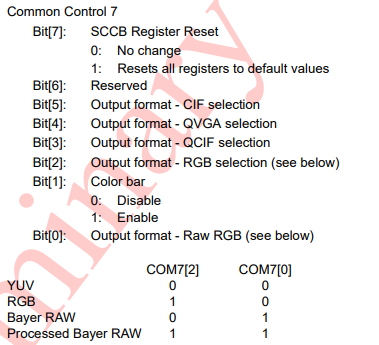
\includegraphics[scale=0.9]{com72}
		\caption{0x12 COM7}
		\label{fig:com72}
	\end{figure}
	\\
	
	\texttt{ov\char`_config} sends out register configurations one by one. There are 0xC9 registers from the data sheet. The most important register is 0x12 COM7 (the name of the register), shown in Figure \ref{fig:com72}. With COM7, color mode between YUV and RGB565 can be toggled. The exact configuration has been copied from the Linux kernel, after understanding the C code \cite{reg6} and filtering out the registers that I need.
	\begin{figure}[h]
		\centering
		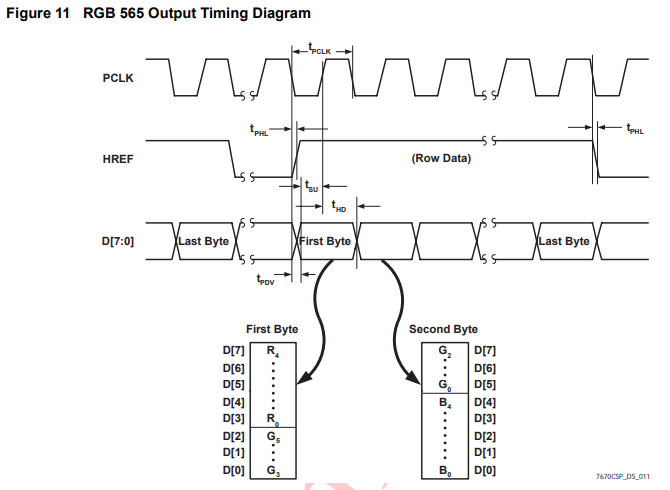
\includegraphics[scale=0.8]{rgb565}
		\caption{Waveform of pixel transfer}
		\label{fig:rgb565}
	\end{figure}
	\texttt{ov\char`_capturer} is purely passive, it responds to pixel clock from the camera. Each pixel is transferred in 2 clocks (Figure \ref{fig:rgb565}), so a shift register is used to save the data from the first clock.\begin{displayquote}
	\textbf{ov\_capturer.vhd:42}: \texttt{shift\_reg(15 downto 0) <= shift\_reg(7 downto 0) \& OV\_DATA}
	\end{displayquote}
	The coordinate is incremented roughly every 2 clocks (roughly because there is no data transfer for line increments, please refer to VGA in Technical Background), until the whole frame is refreshed. For every pixel, the capturer writes it to the first buffer (\texttt{frame\char`_buffer\char`_y}).
	\\
	
	\texttt{kernel3\char`_controller} shifts coordinates every 9 clocks. Within these 9 clocks, it visits the 8-neighbor, and itself, from left to right, top to bottom, shown in Figure \ref{fig:lefttoright}.
	\begin{figure}[h]
		\centering
		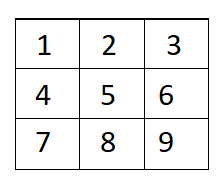
\includegraphics[scale=0.9]{lefttoright}
		\caption{The order that the controller visits}
		\label{fig:lefttoright}
	\end{figure} There are border detections, that if a neighbor goes out of bound, the output coordinate becomes the starting pixel itself.
	\\
	
	As stated before, each pixel from the camera arrives every 2 cycles. But for this controller it needs to consider 9 times more pixels. Luckily the controller is separated from the camera, it can be fed with the fastest clock available from the ZedBoard (100 MHz), and deal with one of the 9 pixels per clock, with a frame buffer in between.
	\\
	
	That's why the first frame buffer exists. Even if the clocks are in the same frequency, the buffer is still needed because the clocks may not be in phase, since one of them is from an external source. Imagine the controller trying to request the pixel row X column Y, but the camera sending the pixel at row X' column Y'. It will not work. Instead, the controller simply requests the pixel content from the frame buffer, and the camera can update this frame buffer independent of what the controller is doing.
	\\
	
	The frame buffer does not need to be manually implemented. It has been done by Xilinx Vivado already, in the form of an Intellectual Property core (IP core). IP core resembles the library concepts in the world of software, that the design within the core can be treated as a black-box. What was left to be done was to generate this IP core, and configure it via the Vivado IP wizard. Configuration includes, but not limited to, the capacity of the buffer. The wizard will then generate skeleton code to be pasted within my code, to avoid linking errors. For example, please refer to \textbf{fyp.vhd:67}.
	\\
	
	Some IP cores need a paid license to be used. However the buffer being used in this project is free of charge.
	\\
	
	In other literature, buffer may be referred as first-in-first-out (FIFO), or block RAM  (BRAM). It is a commonly seen component in FPGA development, when there is a component that needs signal transfer from another component, but they are running different clocks. In this case, the camera is in pixel clock 25 MHz, and the controller is in clock 100 MHz.
	\\
	
	\texttt{kernel3\char`_controller} gives the address to the first buffer, the buffer returns the pixel value to \texttt{kernel3\char`_convolutor}. The controller also sends a state number to convolutor, so that the convolutor knows which matrix entry it should multiply the pixel with (1 of the 9 pixels).
	\\
	
	For every 9 cycles, a pixel’s calculation has been finished by the convolutor, and the result is written to the second buffer (\texttt{frame\char`_buffer\char`_sobel\char`_y}), for VGA to grab. That is because VGA is not running in 100 MHz clock, but 25 MHz clock.
	\\
	
	In the current system, 2 convolutor instances are fed with the Sobel kernels \cite{sobel}
	\begin{align*}
		G_x&=
		\begin{pmatrix}
			1&0&-1\\
			2&0&-2\\
			1&0&-1
		\end{pmatrix},\\
		G_y&=
		\begin{pmatrix}
			1&2&1\\
			0&0&0\\
			-1&-2&-1
		\end{pmatrix}.
	\end{align*}
	
	So, the one convolutor component has been instantiated twice. One for the calculation of the convolution result by $G_x$, one for $G_y$.
	\\
	
	Since there are two components, but just one frame buffer for the VGA \texttt{frame\char`_buffer\char`_sobel\char`_y}, the two results are combined with some glue code.
	\\
	
	 Technically, these two resultant values should be squared, added together then taken the square root
	\begin{align*}
		G&=\sqrt{{G_x}^2+{G_y}^2}.
	\end{align*}
	And then, $G$ should be bounded if it exceeds the minimum or the maximum. This can happen, because observe for $G_x$ and $G_y$, the resulted value can be 4 times the maximum value of a pixel, when the negative entries are multiplied with zero values (i.e., black pixels).
	\begin{align*}
		G&:=\text{min}(\text{PixelValue}_\text{max}, G)\\
		G&:=\text{max}(\text{PixelValue}_\text{min}, G)
	\end{align*}
	
	However, the initial implementation divides the result by 4, as a measure of normalization (which would then be changed),
	\begin{align*}
		G_x&:=\frac{G_x}{4}\\
		G_y&:=\frac{G_y}{4},
	\end{align*}
	which is technically incorrect. These two values are then taken the absolute value and then averaged, instead of taken the squares and square root.
	\begin{align*}
		G&=\frac{\left| G_x \right| +\left| G_y \right|}{2}.
	\end{align*}
	
	This is obviously not the ``correct'' way to implement the Sobel kernel, however implementing square root on an FPGA is too challenging for my current skill level. Therefore, averaging was chosen, as it considers both $G_x$ and $G_y$, and also stays reasonable (from my point of view). The original bound when the resultant value exists the maximum/minimum is not mathematically rigorous anyway.
	\\
	
	However, this resulted in an almost black screen, since the resulted values were too small after $G_x$ and $G_y$ are being divided by 4. Originally, the division by 4 was then taken away and re-tested, but it produced so much noise (Figure \ref{fig:real1}) due the quality of the camera\begin{figure}[h]
		\centering
		\includegraphics[scale=0.15]{real1}
		\caption{Very noisy}
		\label{fig:real1}
	\end{figure}. Instead of thinking that the noise comes from incorrect implementation of the Sobel kernel and indeed came from the camera, this was verified by pointing the camera to a blank paper, in which purple dots (Figure \ref{fig:real2}, \ref{fig:real3}) can be seen and indeed form a circle. This matches the noise pattern shown in figure \ref{fig:real1}.
\begin{figure}[h]
		\centering
		\includegraphics[scale=0.09]{real2}
		\caption{Purple dots despite shooting at a blank paper}
		\label{fig:real2}
	\end{figure}
\begin{figure}[h]
		\centering
		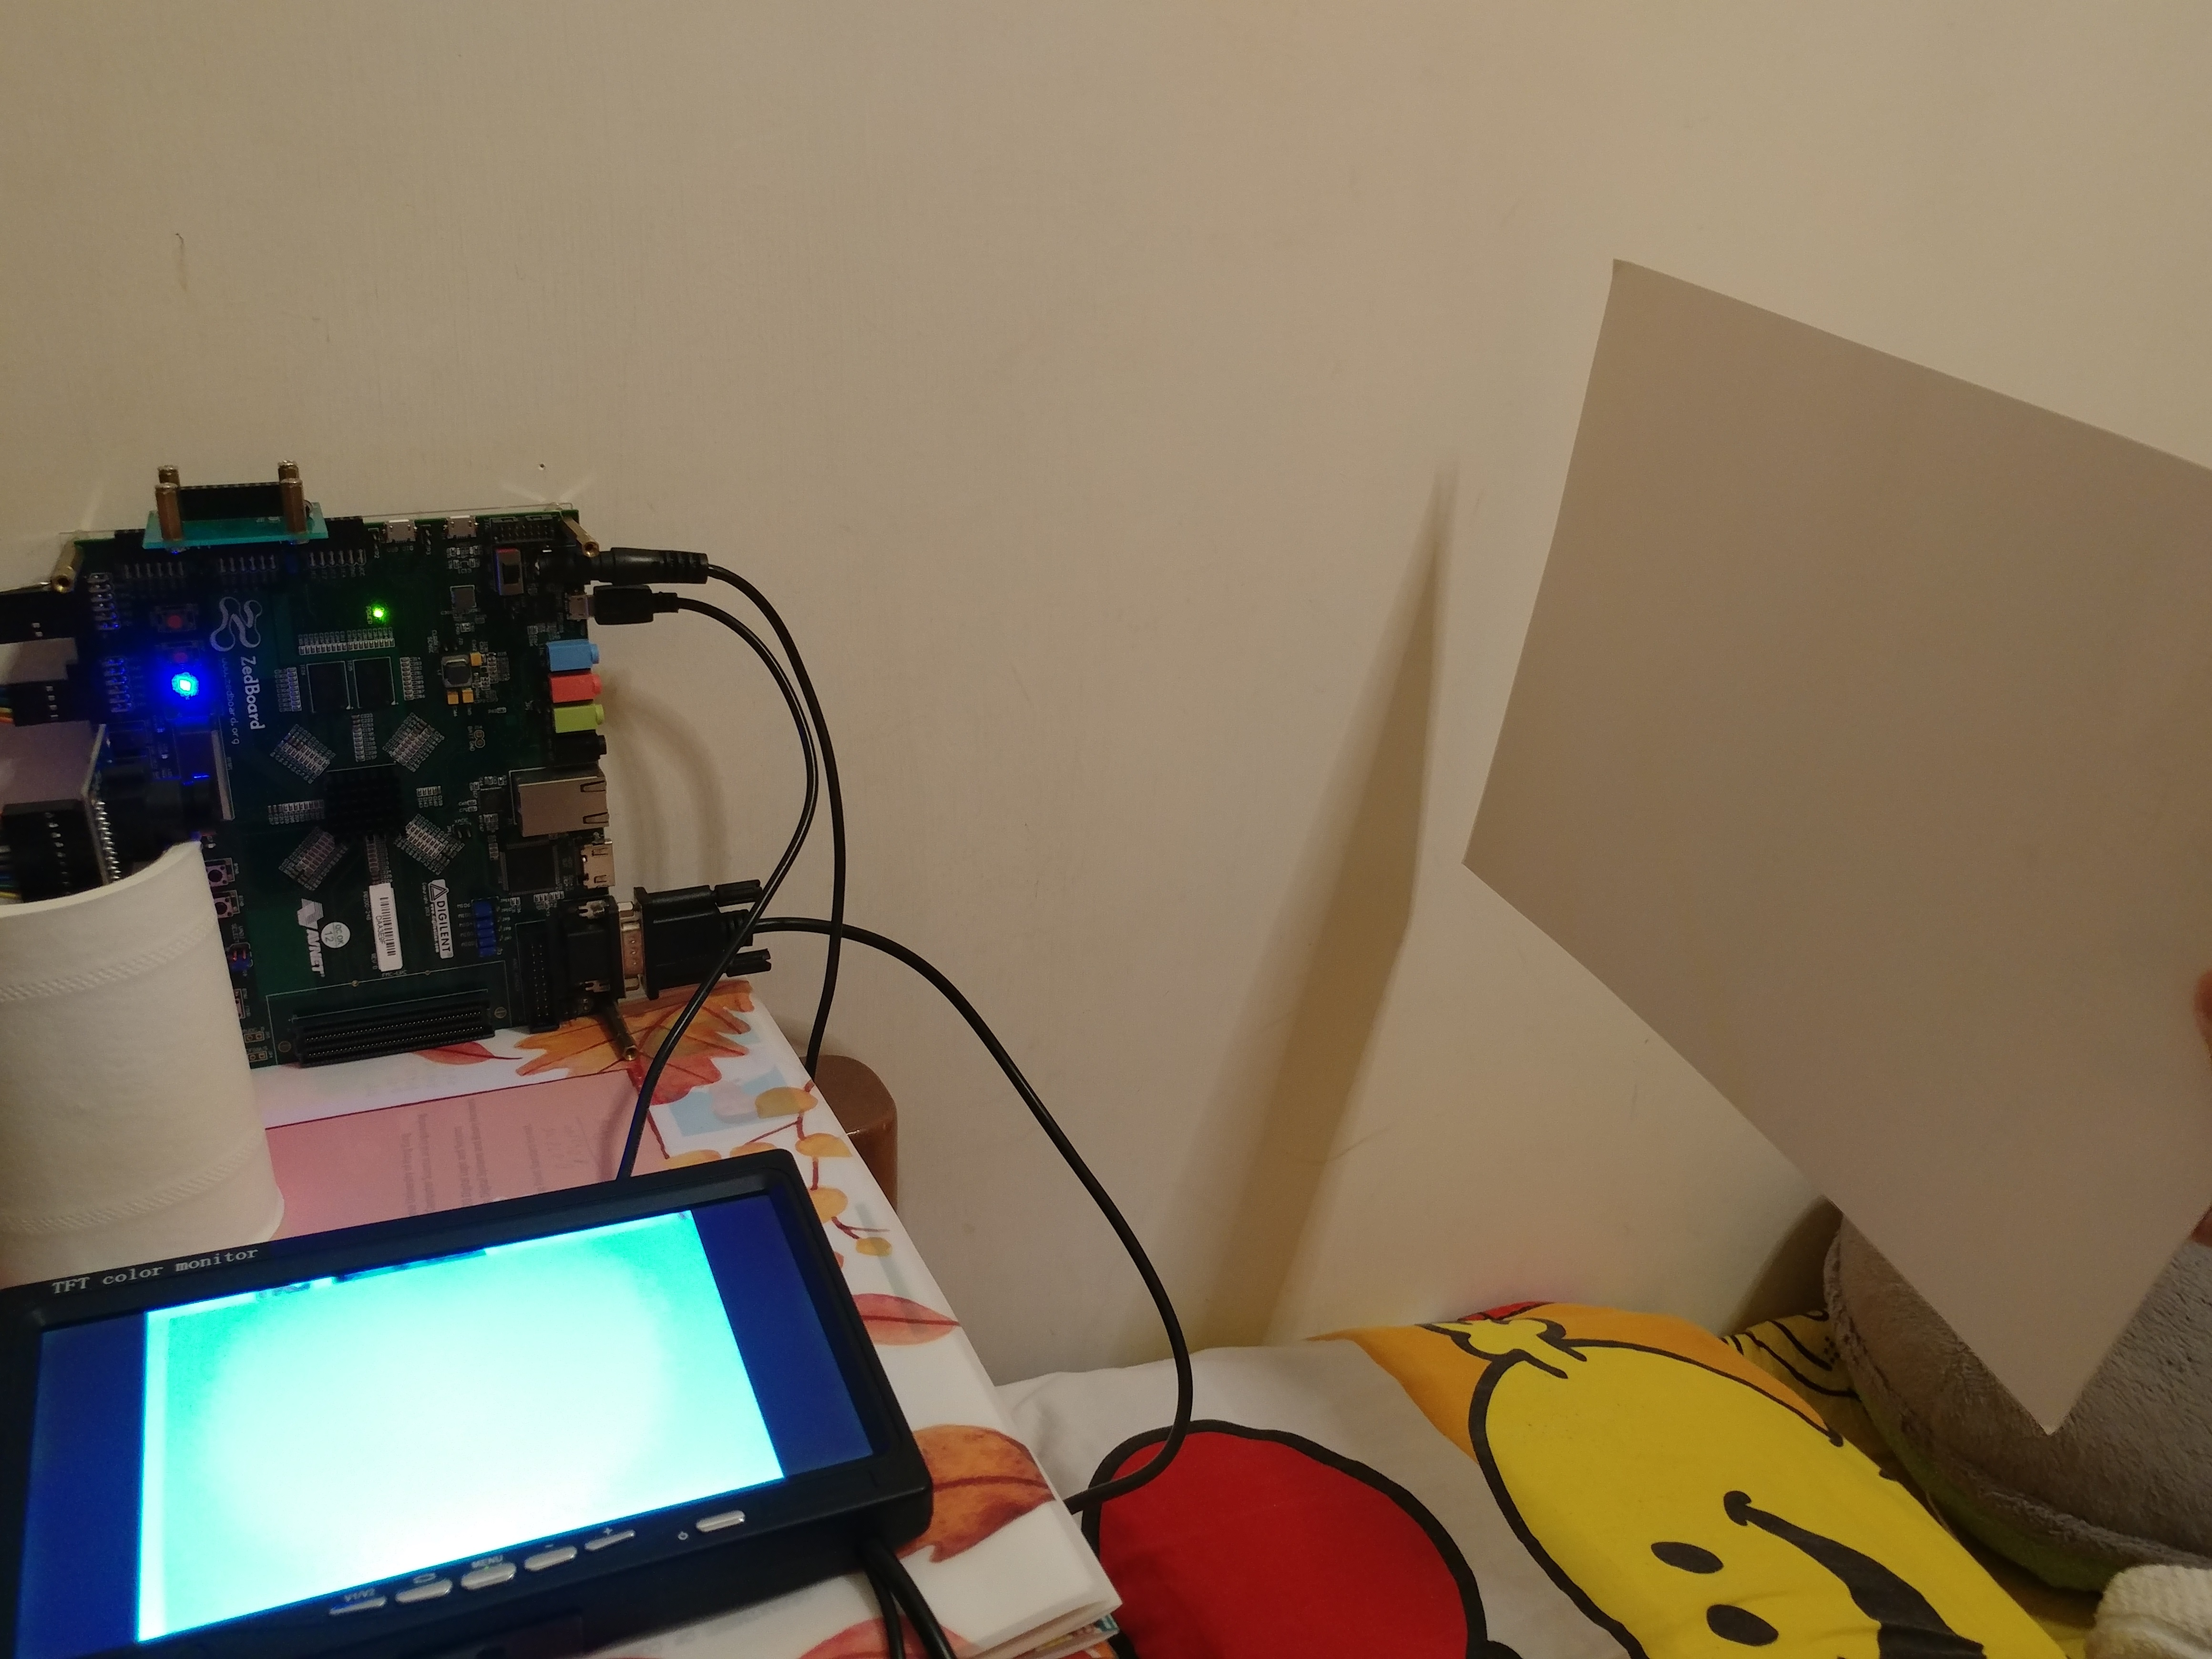
\includegraphics[scale=0.09]{real3}
		\caption{It is indeed the white paper}
		\label{fig:real3}
	\end{figure}
	\\
	
	To deal with this noise issue, an additional Gaussian blur filter 3x3 
	\begin{align*}
		\frac{1}{16}
		\begin{pmatrix}
			1&2&1\\
			2&4&2\\
			1&2&1
		\end{pmatrix}
	\end{align*}
	was tried applying, i.e., having another processing after the Sobel operation with another buffer in-between. Unfortunately, it made no difference.
	\\
	
	Finally, the current implementation mixes both the ``official'' approach and my approach, by first taking the absolute value, then dividing, multiplying back, and the final result is then bounded.
	\begin{align*}
		G_x&=4\left\lfloor{ \frac{1}{4}\left |
		\begin{pmatrix}
			1&0&-1\\
			2&0&-2\\
			1&0&-1
		\end{pmatrix}\right|} \right\rfloor
		,\\
		G_y&=4\left\lfloor{ \frac{1}{4}\left |
		\begin{pmatrix}
			1&2&1\\
			0&0&0\\
			-1&-2&-1
		\end{pmatrix}\right|} \right\rfloor
		.\\
		G&:=\frac{G_x+G_y}{2}\\
		G&:=\text{min}(\text{PixelValue}_\text{max}, G)\\
		G&:=\text{max}(\text{PixelValue}_\text{min}, G)
	\end{align*}
	
	 This implementation removes all the noise, because of the division, $\frac{1}{4}$, (implemented as shifts), and the floor operation $\lfloor\hspace{1ex} \rfloor$, making them zero. Which means the smaller values, which mostly consisted of noises, are filtered away in effect, and the whole result is amplified again.
	\\
	 
	 However, some tiny portions of the supposedly edges are also lost in this process (Figure \ref{fig:real4}).
\begin{figure}[h]
		\centering
		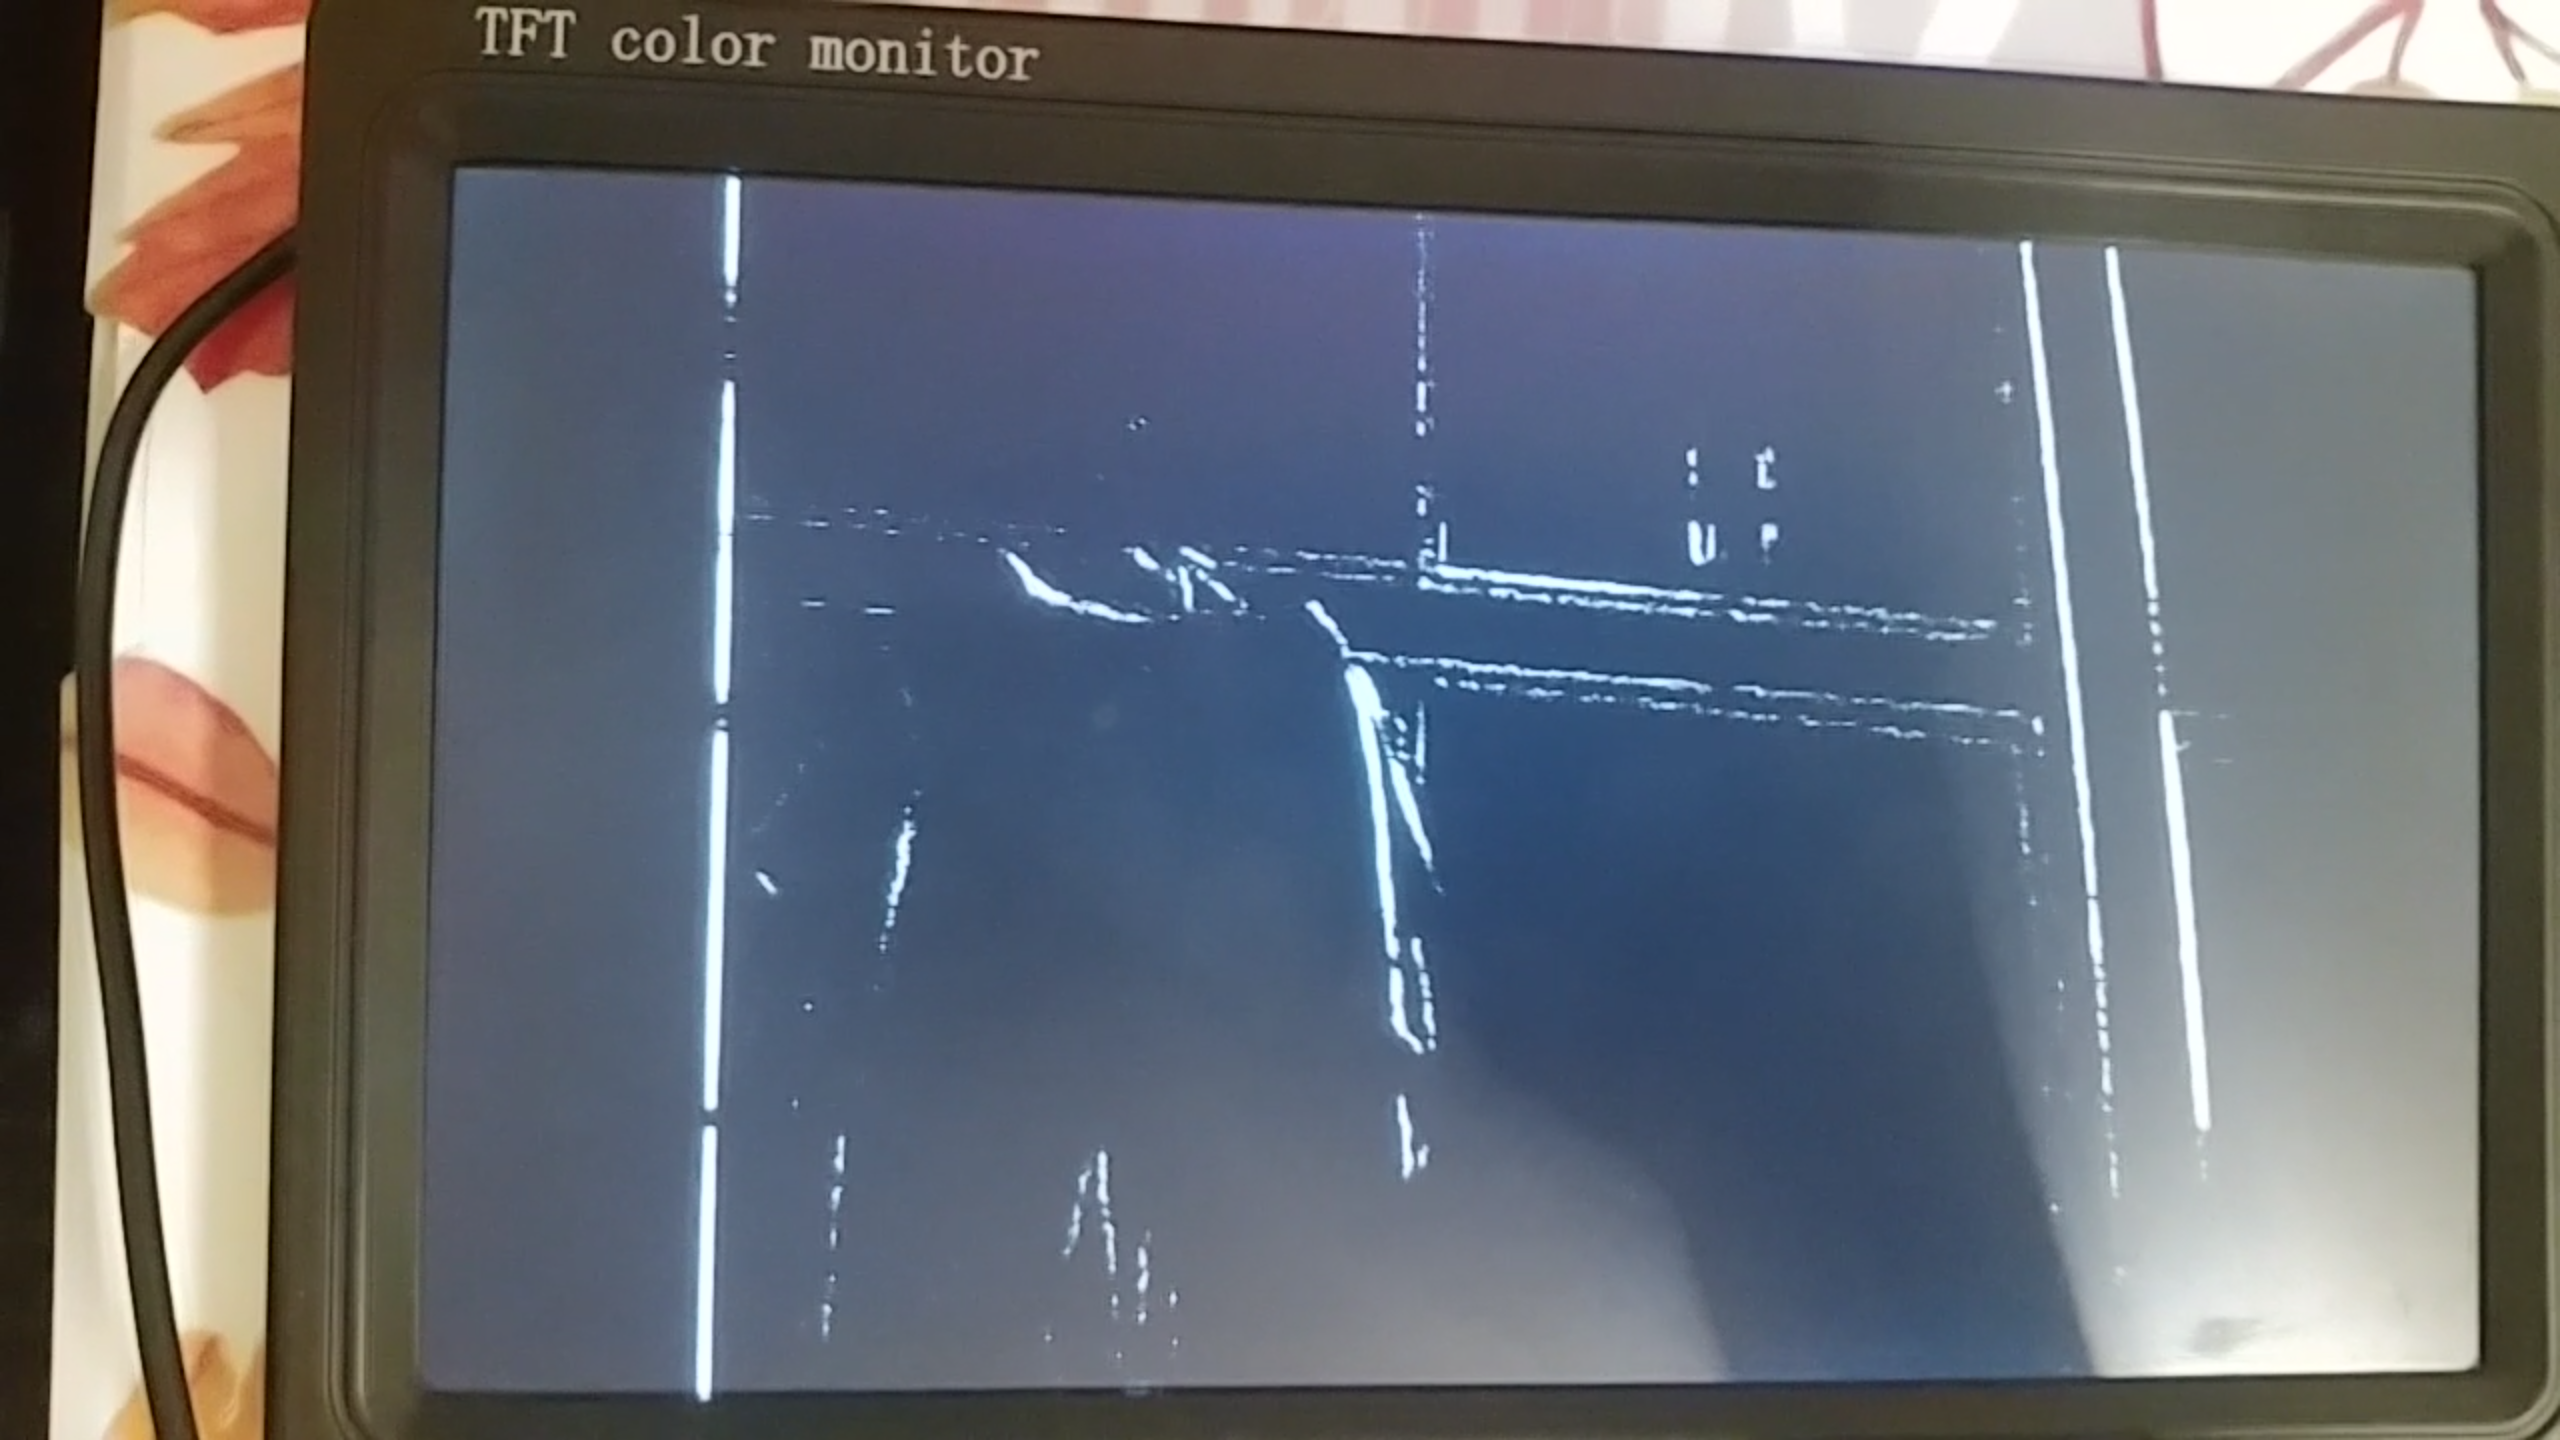
\includegraphics[scale=0.15]{real4}
		\caption{Some edges lost}
		\label{fig:real4}
	\end{figure}This result comes from the fact that the camera cannot produce highly distinct colors for real edges.
	\\
	 
	 To prove this, if the camera was fed by black and white 2D codes, which its decoding is something that hopefully can be done by my FPGA skill in the next semester, the edges are very clean (Figure \ref{fig:real5}, \ref{fig:real6}).
\begin{figure}[h]
		\centering
		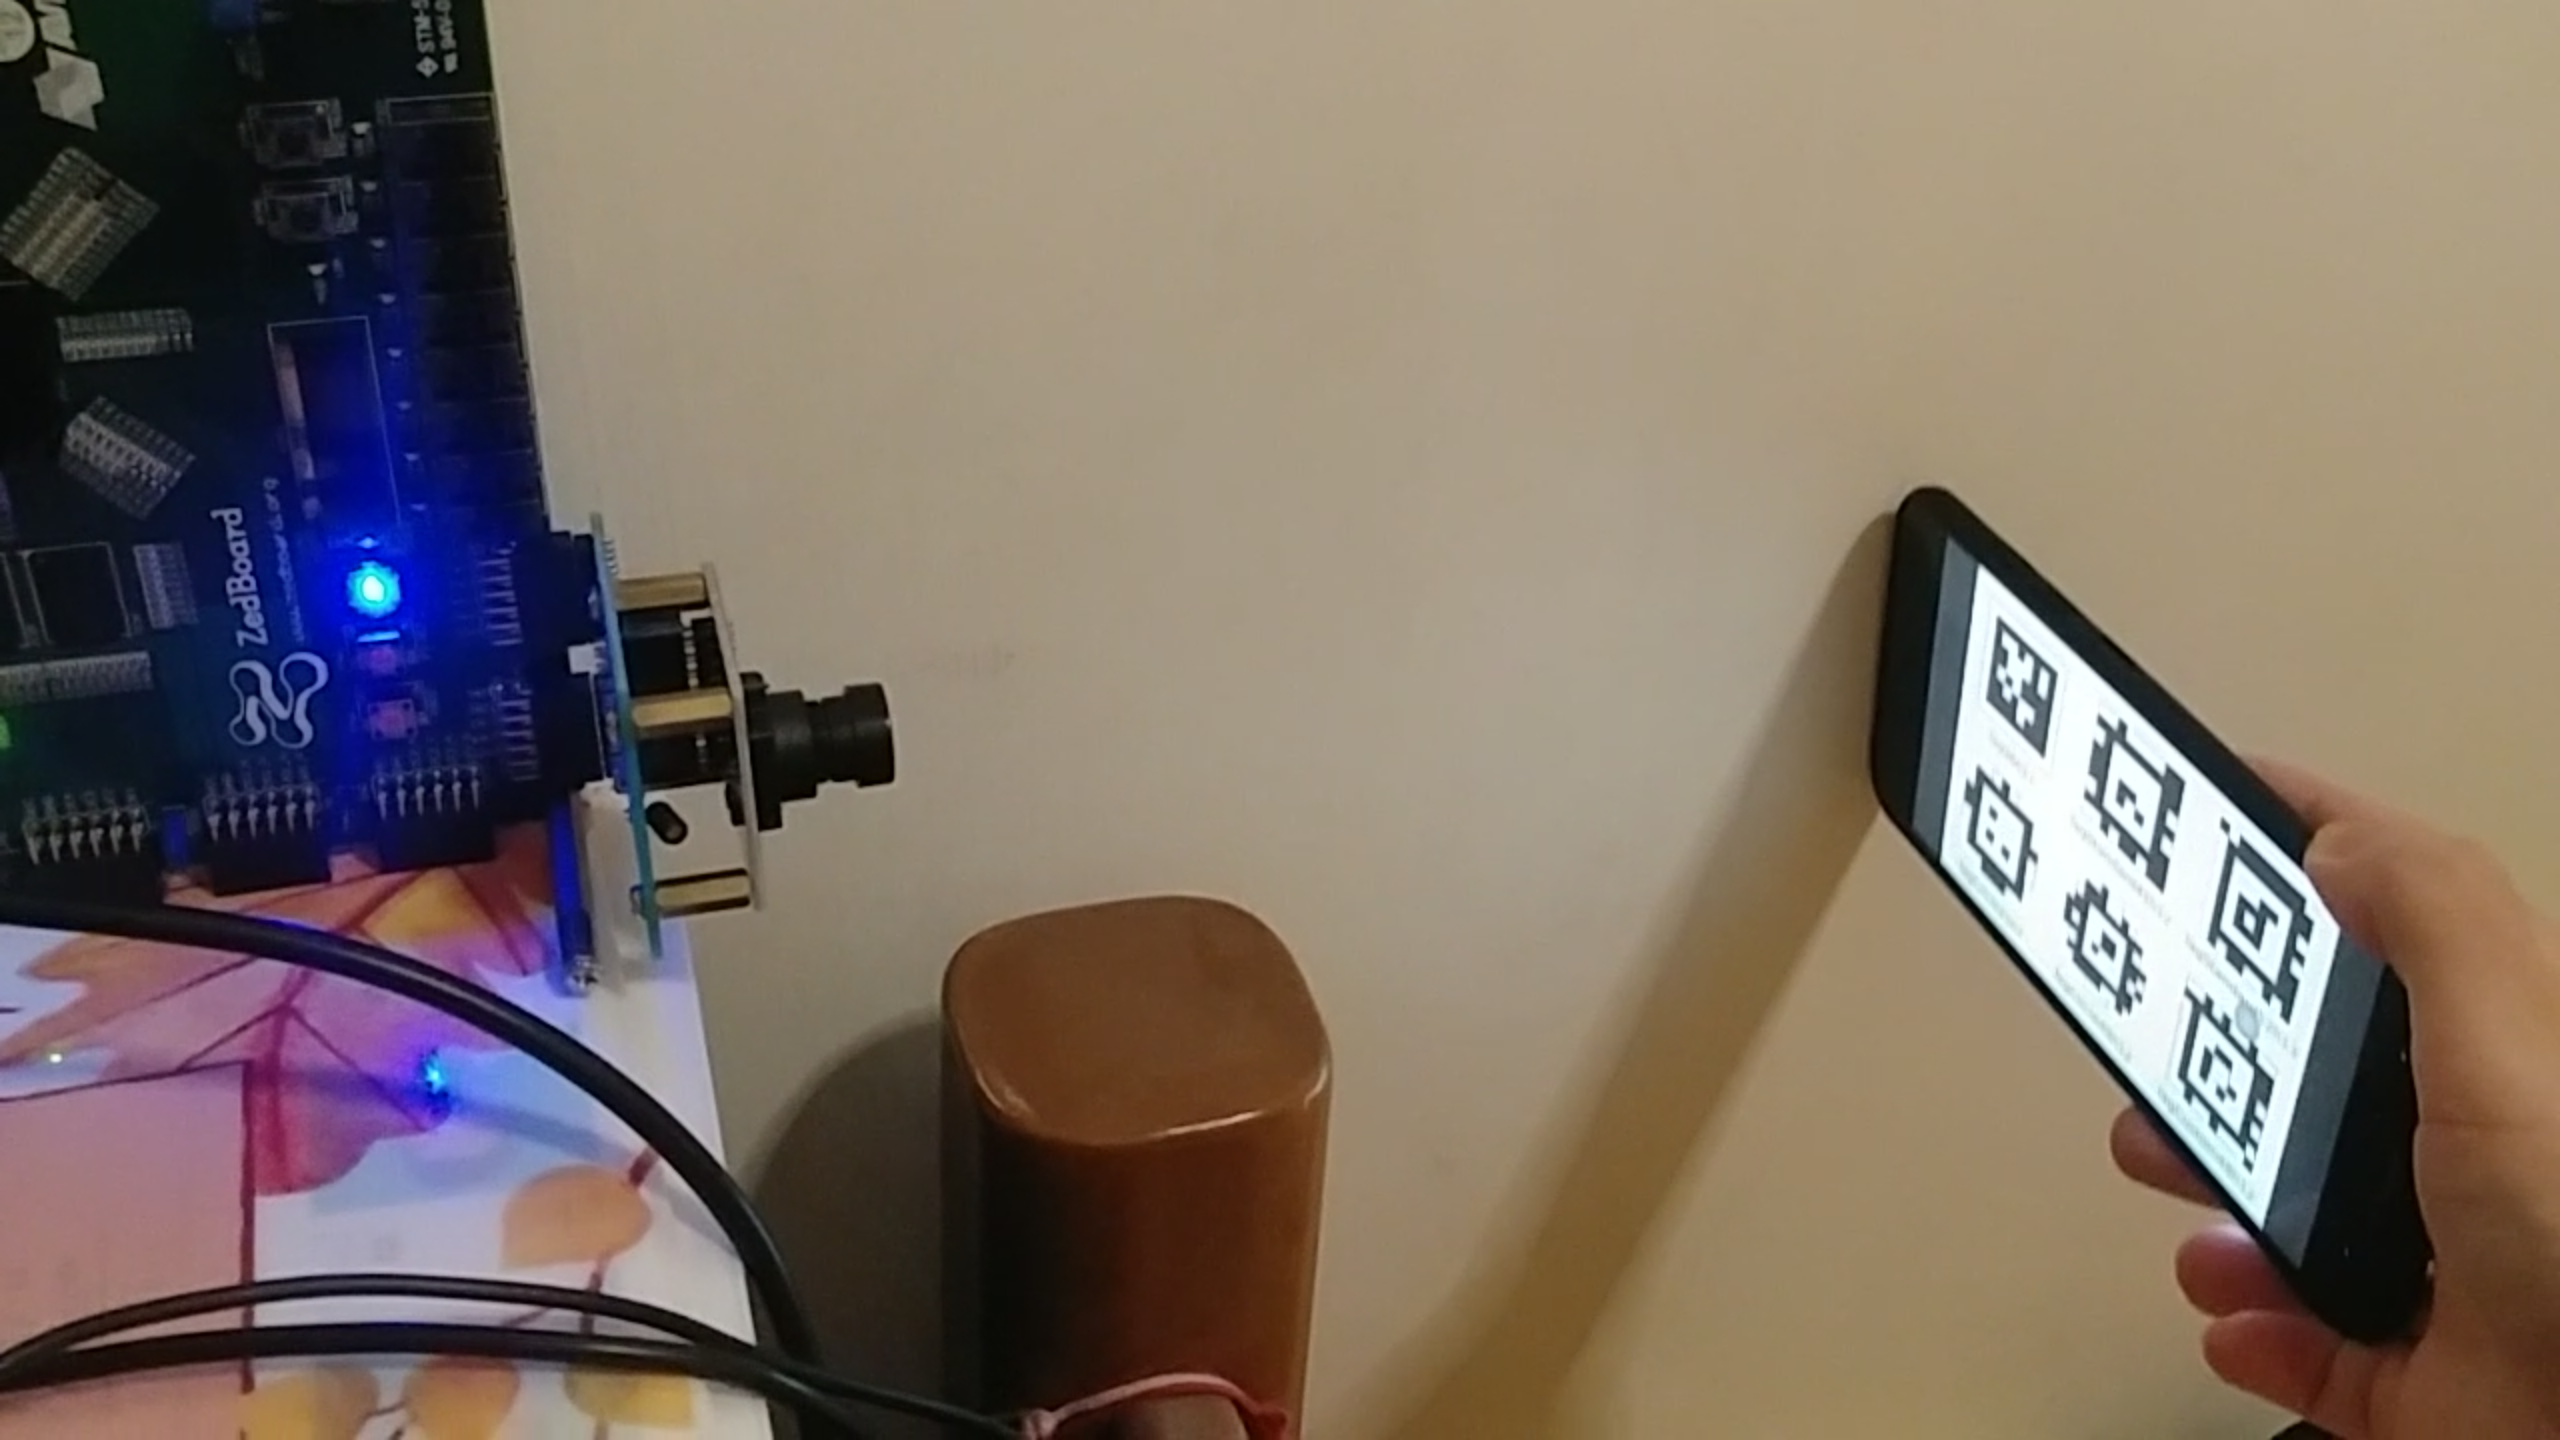
\includegraphics[scale=0.15]{real5}
		\caption{AprilTags}
		\label{fig:real5}
	\end{figure}
\begin{figure}[h]
		\centering
		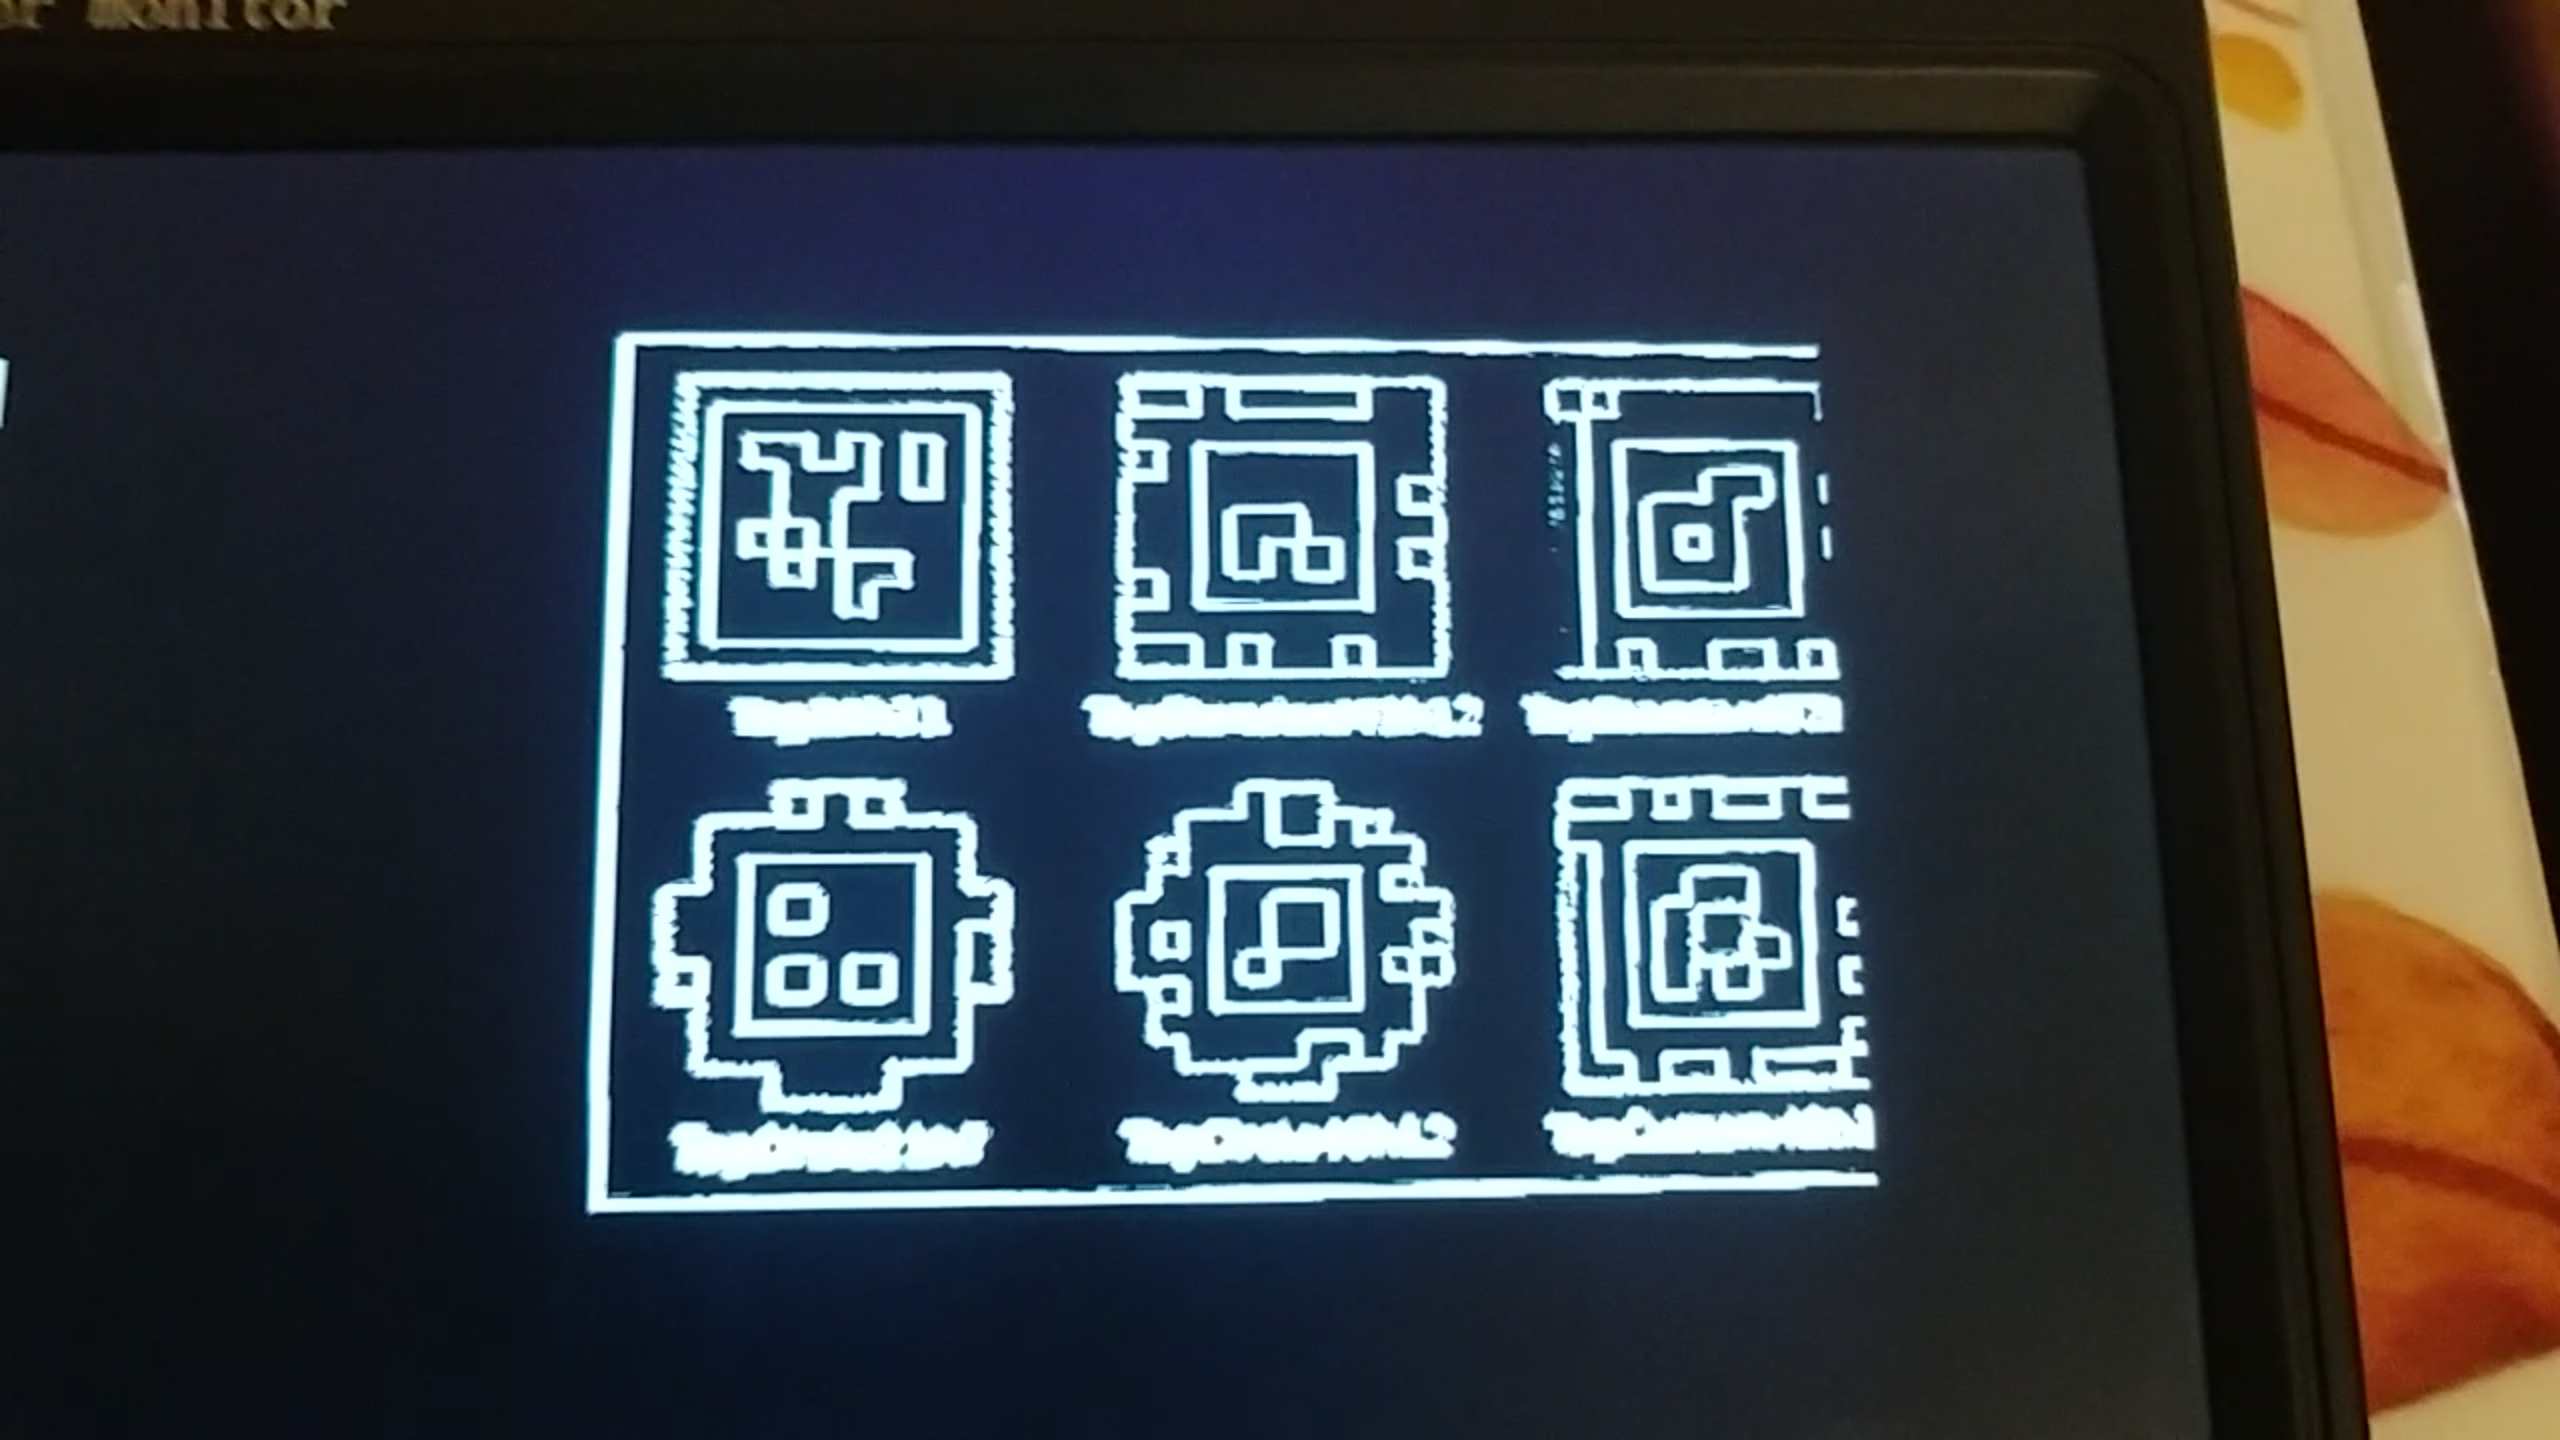
\includegraphics[scale=0.15]{real6}
		\caption{Clean output}
		\label{fig:real6}
	\end{figure}
	\\
	
	Finally, \texttt{vga} pulls data from the second buffer, and output the appropriate VGA waveforms, specified in the section Technical Background.
	\\
	
	The components' code are not screenshoted and put here, due to them being too long and not meaningful for the report. For actual code, the git repository can always help, which contains readable code.
	\\
	
	In short summary, the camera’s SCCB runs at a period of 5600 ns. The camera's pixel clock runs at 25 MHz, the convolution runs at 100 MHz, and standard VGA runs at 25 MHz. Buffers are connected in between when the clock frequencies do not match.
	\newpage\section{Difficulties}
	A huge amount of time has been spent on dealing with the camera. The main problem comes from the poor quality of the data sheet. Before getting hands on the camera, I thought the camera would either 1) work, and produces ideal/usable frames, or 2) produce no output at all. Obviously, now I know how wrong I was. There are numerous registers sets \cite{reg1}\cite{reg2}\cite{reg3}\cite{reg4}\cite{reg5} for the OV7670, but none of them works perfectly (at least to the current extent) on the ZedBoard. Most of them contradict with each other, probably due to different units which the camera are being controlled from. Some configurations do work (have a video output), but they either have weird colors and white balance, or unbearable noise levels (did not take pictures at this stage, sorry). I tried fixing the configurations on my own, but there are many camera-specific abbreviations on the data sheet that I could not understand. There are also just too many registers.
	\\
	
	Finally, the Linux set of configurations \cite{reg6} were found and adapted. Even that did not work on the FPGA initially, but the artifacts were sorted out eventually. Comments from the Linux kernel source code \cite{reg6} have been encouraging though: 
	\begin{displayquote}
		\textbf{Line 200}: (the registers) do not always make complete sense to humans\\
		\textbf{Line 384}: Extra-weird stuff\\
		\textbf{Line 1045}: a pain in the \_\_\_\\
		\textbf{Line 1289}: Weird crap\\
		\textbf{Line 1466}: If one believes the data sheet, …
	\end{displayquote}
	So at least someone else in the world had been sharing the same frustration as me.
	\\
	
	Apart from the problems documented in the kernel code, another problem I find is that if COM7 is sent 0x80 (soft reset) 3 times in a row, the camera will pass out immediately. If only one COM7 command is sent out, it likely still will not work, due to the camera needing a settling time of 1 ms. That is why hardware reset is being used, controlled by a button with debouncing. Normally a button will be pressed for longer than 1 ms.
	\\
	
	Also, two registers 0x17 HSTART and 0x18 HSTOP behave weirdly. The meaning of these two registers are in figure \ref{fig:hstart}.
	\begin{figure}[h]
		\centering
		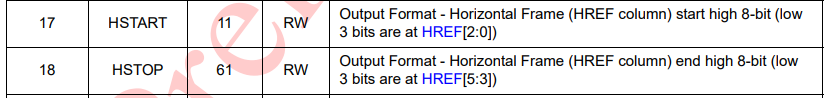
\includegraphics[scale=0.68]{hstart}
		\caption{HSTART description from the data sheet}
		\label{fig:hstart}
	\end{figure} In my interpretation, these two registers control the horizontal width of the image produced by the camera, as the host device may want to accept some horizontal resolution less than 640. The default values of them, i.e., when these two registers are not being programmed, will be 0x11 and 0x61. This makes sense, because HSTART is less than HSTOP.
	\\
	
	However, in the current system, HSTART and HSTOP have the value of 0x13 and 0x01 respectively. They are followed from the Linux configuration. I do not understand the reason of HSTART greater than HSTOP, but it works.
	\\
	
	Another notable data sheet bug is, if the SCCB runs well below the maximum frequency 400 KHz (shown in Figure \ref{fig:sccbtiming} from the data sheet)
	\begin{figure}[h]
		\centering
		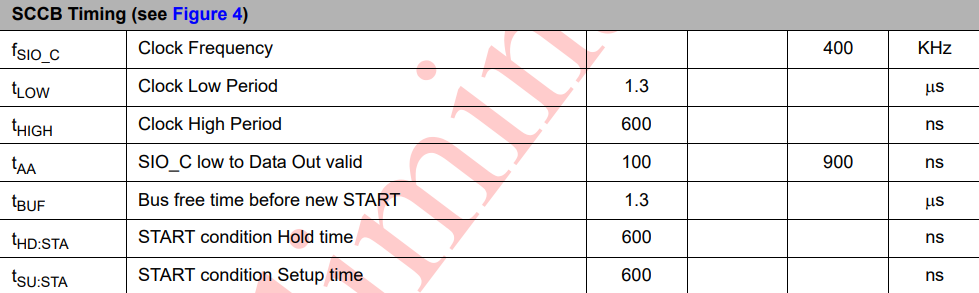
\includegraphics[scale=0.57]{sccbtiming}
		\caption{According to the data sheet, the frequency of SCCB can go up to 400 KHz = 2500 ns.}
		\label{fig:sccbtiming}
	\end{figure}, i.e., well above minimum period 2500 ns, stated in the data sheet, at 2800 ns, the camera will not work. The current implemented SCCB speed runs at 5600 ns.
	\\
	
	To make matters worse, this camera sensor by itself has high variations. The first sensor that I borrowed from the laboratory straight up did not work. The second did work but was not great, and it was not until the third one which has been bearable. Before that, whenever there was a problem, I could not tell if the problem was from my logic, from the configurations, or from the camera.
	\\
	
	When it comes to difficulties not related to the camera, it mainly has to do with me being a newbie in hardware coding. I have to think in clock cycles, instead of sequential instructions, which is not something I have been used to. VHDL’s syntax being new to me does not help either.
	\\
	
	Even though I have heard VGA and I\textsuperscript{2}C (which is very similar to SCCB) before, I did not know how they work. In the end, everything has been rewritten, because I could not figure out how to remove problems from different code snippets found online. Which means that now I know how the protocols work. If I had taken the computer engineering course about FPGAs, these stuff may have been solved quicker.
	\\
	
	A few testbenches have been written to verify the code, but they have only been for stuff that I know how to test. I did not know how to test bugs related to the camera, or frame buffers. For example, the convolution module has been written in a short time, but for a long time the video output has been blank (it turned out to be yet again, some problems related to the camera), and I got confused.
	\\
	
	In terms of logistic difficulties, they were relatively minor. Back in May, I borrowed another FPGA evaluation board ZCU102. Although it is more powerful, it lacks basic I/O that I need, such as VGA. Eventually I returned it, and settled for the ZedBoard.
	\\
	
	Then, for the first few weeks of the semester, I needed to go back to the laboratory because I did not realize VGA monitor can be borrowed. When I was at home, I read how QR codes \cite{utube1}, DataMatrices\cite{utube2} and AprilTags are decoded \cite{apriltag}\cite{apriltag2}, and also how certain algorithms can be implemented on FPGAs. Some ideas of FPGA algorithms to detect these codes have also been appearing in my mind. But the implementation side of things have been lagging behind.
	\\
	
	Long compilation and synthesis time from Vivado also contributed to the slow implementation progress (Figure \ref{fig:vivado}). It is a lot longer than what I am used to, being able to compile software code in a minute.
	\\
	
	This has been a \emph{very} time-consuming issue, as every time I needed to try out a different register settings for the camera, I needed to re-synthesis the whole project. It also increases frustration level.
	\begin{figure}[h]
		\centering
		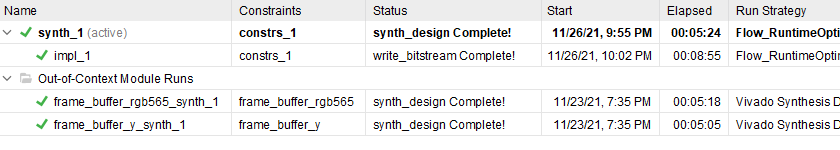
\includegraphics[scale=0.68]{vivado}
		\caption{A single Vivado synthesis takes 14 mins}
		\label{fig:vivado}
	\end{figure}
	\section{Future Work}
	The most immediate target is to ease debugging. A new testbench should be written, such that it takes a picture file from the computer, process the file with the HDL modules, and write the file back to disk. This way, slow synthesis can be avoided more often.
	\\
	
	The second target is to figure out how to store the frame buffer on the on-board DRAM. Right now, frame buffers are on block RAM, but block RAM on this SoC is rather limited. It is not sure at this point, if the DRAM is wired to the FPGA, or it is just limited to the processing system.
	\\
	
	FPGA techniques and algorithms should be the focus of the next semester. Traditional sequential algorithms, such as finding the trigonometry function of a floating point number, or finding a patch of similar pixels with BFS or DFS, cannot be easily implemented on FPGAs. A few techniques, namely connected component analysis \cite{cca} and CORDIC have been found, and may be useful (and difficult).
	\\
	
	Also, hopefully a way to generate the whole Vivado project using a single Tcl script will be figured out. Vivado generates a lot of cache files, and they are not being friendly to the version control system. Currently, the whole project directory is being tracked, with only primitive git ignore files.
	\\
	
	Lastly, a VGA library to output text and basic graphics will be nice and interesting, if it can be found online or written on my own. Depending on the actual benefits, for example its usefulness on debugging, this may be skipped.
	\newpage\section{Conclusion}
	A complete system with Sobel edge detection has been developed in VHDL, as a baseline for further algorithmic development. Lots of hardware problems have been solved, and should no longer be encountered.
	\section{Acknowledgment}
		Sincere sorry for all the delays I have caused, including the late presentation. I failed to keep good track of deadlines and reports.
	\\
		
		I sincerely thank Dr. Sum and Prof. Lee for their understandings, for dealing with my FYP, and for needing to read my report again.
	\newpage
	\renewcommand{\baselinestretch}{2}\normalsize
	\begin{thebibliography}{99}
        \bibitem{vga}
            MIT 6.111 Lab Kit: \textit{VGA Video}, \\ \longvar{https://web.mit.edu/6.111/www/s2004/NEWKIT/vga.shtml}
            
        \bibitem{rpi}
            Joshua Hrisko: \textit{Image Processing Object Detection with Raspberry Pi and Python}, \\ \longvar{https://makersportal.com/blog/2019/4/23/image-processing-with-raspberry-pi-}\\\longvar{and-python-part-ii-spatial-statistics-and-correlations}            
            
	\bibitem{ovdatasheet}
	OV7670 Data Sheet \\ \longvar{http://web.mit.edu/6.111/www/f2016/tools/OV7670_2006.pdf}
	\bibitem{sccbdatasheet}
	SCCB Reference\\ \longvar{https://www.waveshare.com/w/upload/1/14/OmniVision_Technologies_Seril_Camera_Control_Bus\%28SCCB\%29_Specification.pdf}
	
	\bibitem{sobel}
	Wikipedia: \textit{Sobel Operator}\\ \longvar{https://en.wikipedia.org/wiki/Sobel_operator}
    
	\bibitem{utube1}
	How to Decode a QR Code by Hand: \\ \longvar{https://www.youtube.com/watch?v=KA8hDldvfv0}
	\bibitem{utube2}
	How to Decode a DataMatrix Code by Hand: \\ \longvar{https://www.youtube.com/watch?v=w0xVd2xXySo}
	\bibitem{apriltag}
	Edwin Olson: \textit{AprilTag: A robust and flexible visual fiducial system}\\ \longvar{https://april.eecs.umich.edu/media/pdfs/olson2011tags.pdf}
    
	\bibitem{apriltag2}
	Ethan Tola: \textit{Real-Time UAV Pose Estimation and Tracking using FPGA Accelerated April Tag}\\ \longvar{https://scholarworks.rit.edu/cgi/viewcontent.cgi?article=11999&context=theses}
	
	\bibitem{cca}
	D.G. Bailey, C.T. Johnston: \textit{Single Pass Connected Components Analysis}\\ \longvar{http://sprg.massey.ac.nz/pdfs/2007_ivcnz_282.pdf}
	
	
	\bibitem{reg1}
	Register Set 1: \\ \longvar{https://web.archive.org/web/20150402065629/http://hamsterworks.co.nz/mediawiki/index.php/Zedboard_OV7670}
	\bibitem{reg2}
	Register Set 2: \\ \longvar{https://github.com/jonlwowski012/OV7670_NEXYS4_Verilog/blob/master/ov7670_registers_verilog.v}
	\bibitem{reg3}
	Register Set 3: \\ \longvar{https://github.com/iwatake2222/DigitalCamera_STM32/blob/master/Src/driver/ov7670/ov7670Reg.h}
	\bibitem{reg4}
	Register Set 4: \\ \longvar{https://92zo.at.webry.info/201301/article_2.html}
	\bibitem{reg5}
	Register Set 5: \\ \longvar{https://github.com/adafruit/Adafruit_OV7670/blob/master/src/ov7670.c}
	\bibitem{reg6}
	Register Set 6: \\ \longvar{https://github.com/torvalds/linux/blob/master/drivers/media/i2c/ov7670.c}
	
	
    \end{thebibliography}
\end{document}
